%the entire chapter is typed and edited
% all footnotes have been included
\باب{تفاعل موج}\شناخت{باب_تفاعل_موج}
\حصہ{شروڈنگر مساوات} 
فرض کریں   محور   \عددی{x}  پر رہنے کا  پابند ایک ذرہ  جس کی   کمیت  \عددی{m} ہو  پر قوت \عددی{F(x,t)} عمل کرتی ہے  (شکل \حوالہ{شکل_تفاعل_موج_حرکت_یک_بعدی})۔ کلاسیکی میکانیات میں اس ذرے کا مقام \عددی{x(t)}  کسی بھی وقت \عددی{t} پر  متعین کرنا درکار ہوتا ہے۔ ذرے کا مقام جاننے کے بعد ہم اس کا اسراع، سمتی رفتار  \عددی{ v = \tfrac{\dif x}{\dif t} }، معیار حرکت  \عددی{p = mv} یا حرکی توانائی  \عددی{T = \tfrac{1}{2} mv^{2} } یا کوئی اور حرکی متغیر جس میں ہم دلچسپی رکھتے ہوں،     متعین کر سکتے ہیں۔  سوال پیدا ہوتا ہے کہ ہم \عددی{x(t)} کیسے متعین  کریں گے۔ ہم نیوٹن کا دوسرا قانون  \عددی{F=ma}  بروئے کار لاتے ہیں۔ (بقائی نظام جو خوش قسمتی سے خوردبینی سطح پر واحد نظام ہے، میں قوت کو مخفی توانائی\حاشیہد{مقناطیسی قوتوں کے لئے ایسا نہیں ہو گا لیکن یہاں ہم ان کا  تذکرہ  نہیں کر رہے ہیں۔ نیز، اس کتاب میں ہم رفتار کو غیر اضافی \عددی{(v\ll c)} تصور کریں گے۔} پر تفرق لکھا جا سکتا ہے \عددی{F = -\tfrac{\partial V}{\partial x}}،  لہٰذا نیوٹن کا قانون  \عددی{m\tfrac{\dif{\,^2} x}{\dif t^{\,2}} = -\tfrac{\partial V}{\partial x}} لکھا جائے گا۔)   ابتدائی معلومات، جو عموماً لمحہ \عددی{t=0} پر سمتی رفتار یا مقام ہوں گے، استعمال کرتے ہوئے    اس مساوات کے ذریعہ  ہم  \عددی{x(t)} دریافت کر سکتے ہیں۔
 
 \begin{figure}
 \centering
 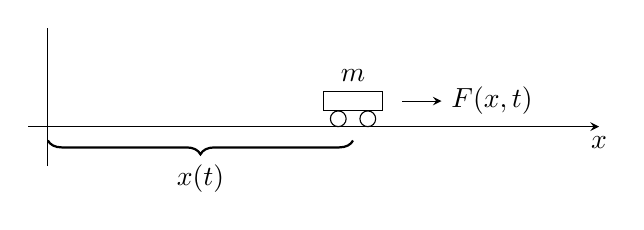
\begin{tikzpicture}
 \pgfmathsetmacro{\r}{0.1}
 \pgfmathsetmacro{\l}{0.75}
 \pgfmathsetmacro{\h}{0.25}
 \pgfmathsetmacro{\s}{3.5}
 \pgfmathsetmacro{\a}{\s+0.25*\l}
  \pgfmathsetmacro{\b}{\s+0.75*\l}
 \draw[-stealth](-0.25,0)--(7,0)node[below]{$x$};
 \draw(0,-0.5)--(0,1.25);
 \draw(\a,\r) circle (\r);
  \draw(\b,\r) circle (\r);
  \draw(\s,2*\r) rectangle ++(\l,\h);
  \draw(\s+0.5*\l,2*\r+\h)node[above]{$m$};
  \draw[-stealth](\s+\l+0.25,2*\r+\h/2)--++(0.5,0)node[right]{$F(x,t)$};
  \draw [decorate,decoration={brace,amplitude=5pt,mirror},yshift=-5pt,thick] (0,0) -- (\s+\l/2,0)node [black,midway,below,yshift=-5pt] {$x(t)$};
 \end{tikzpicture}
 \caption{ایک مخصوص قوت کے پیش نظر ایک "ذرہ" ایک بُعد پر رہتے ہوئے حرکت کرنے پر مجبور ہے۔}
 \label{شکل_تفاعل_موج_حرکت_یک_بعدی}
 \end{figure}
کوانٹم میکانیات اس مسئلے کو بالکل مختلف انداز سے  دیکھتی  ہے۔ اب ہم ذرے کے  \اصطلاح{تفاعل موج}\فرہنگ{تفاعل موج}\حاشیہب{wave function}\فرہنگ{wave function}،  جس کی علامت \عددی{\Psi(x,t)} ہے،   کو \اصطلاح{شروڈنگر مساوات}\فرہنگ{شروڈنگر مساوات}\حاشیہب{Schrodinger align}\فرہنگ{Schrodinger align}:
\begin{align}\label{مساوات_تفاعل_موج_شروڈنگر_الف}
 i \hslash \frac{\partial \Psi}{\partial t} = - \frac{\hslash^{2}}{2m} \frac{\partial \Psi^{2}}{\partial x^{2}} + V \Psi
\end{align}
حل کر کے حاصل کرتے ہیں جہاں  \عددی{i}  منفی ایک \عددی{(-1)} کا جذر  اور  \عددی{\hslash} پلانک  مستقل، بلکہ اصل پلانک مستقل تقسیم  \عددی{2\pi}   ہو گا۔
\begin{align}
 \hslash = \frac{h}{2\pi} = \SI{1.054572e-34}{\joule\second} 
\end{align}
شروڈنگر  مساوات نیوٹن کے دوسرے قانون کا مماثل کردار ادا کرتی ہے۔ دی گئی ابتدائی معلومات ( عموماً \عددی{\Psi(x,0)} )   استعمال کرتے ہوئے  شروڈنگر مساوات،  مستقبل کے تمام اوقات کے لئے، \عددی{\Psi (x,t)} کا  تعین کرتی ہے، جیسے  کلاسیکی میکانیات میں تمام مستقبل اوقات کے لئے  قاعدہ نیوٹن  \عددی{x(t)}  متعین کرتا ہے۔ 
 
%=======================

\حصہ{شماریاتی مفہوم}\شناخت{حصہ_تفاعل_موج_شماریاتی_مفہوم}
تفاعل موج حقیقت میں کیا ہوتا ہے اور یہ جانتے ہوئے آپ حقیقت میں کیا کر سکتے ہیں؟   ایک ذرے کی خاصیت ہے کہ وہ ایک نقطے پر پایا جاتا ہو لیکن ایک تفاعل موج ( جیسا کہ اس کے نام سے ظاہر ہے)  فضا میں پھیلا ہوا پایا جاتا ہے۔ کسی بھی لمحے  \عددی{t} پر یہ\عددی{x} کا تفاعل ہو گا۔  ایک تفاعل ایک ذرے کی حالت کو کس طرح بیان کر پائے گا،   اس کا جواب تفاعل موج کا  \اصطلاح{شماریاتی مفہوم}\فرہنگ{شماریاتی مفہوم}\حاشیہب{statistical interpretation}\فرہنگ{statistical!interpretation} پیش کر کے جناب بارن نے دیا جس کے تحت لمحہ \عددی{t} پر نقطہ \عددی{x} پر ایک ذرہ  پائے جانے کا احتمال \عددی{|\Psi(x,t)|^2}  ہو گا، بلکہ اس کا زیادہ درست روپ\حاشیہد{تفاعل موج خود مخلوط ہے لیکن \عددی{|\Psi|^2=\Psi^*\Psi} ( جہاں \عددی{\Psi^*} تفاعل موج \عددی{\Psi} کا مخلوط جوڑی دار ہے) حقیقی اور غیر منفی ہے، جیسا کہ ہونا بھی چاہیے۔}  درج ذیل ہے۔
\begin{align}\label{مساوات_تفاعل_موج_شماریاتی_مفہوم_الف}
\int_a^b\abs{\Psi(x,t)}^2\dif x=
\begin{cases}
\begin{minipage}{0.25\textwidth}
\RL{
لمحہ \عددی{t} پر \عددی{a} اور \عددی{b} کے بیچ ایک ذرہ کے  پائے جانے کا احتمال
}
\end{minipage}
\end{cases}
\end{align}
احتمال \عددی{|\Psi|^2} کی ترسیم کے نیچے رقبے کے برابر ہو گا۔شکل  \حوالہ{شکل_تفاعل_موج_احتمال_اور_رقبہ}  کی تفاعل موج کے لئے  ذرہ غالباً   نقطہ \عددی{A} پر پایا جائے  گا جہاں \عددی{\abs{\Psi}^2} کی قیمت زیادہ سے زیادہ ہے جبکہ  نقطہ \عددی{B} پر ذرہ غالباً نہیں پایا جائے گا۔

\begin{figure}
\centering
\begin{tikzpicture}
\begin{axis}[small,axis lines=middle,xlabel={$x$},ylabel={$\abs{\Psi}^2$},xmax=7.5,xtick={0.75,1.75,2.5,4,4.75},xticklabels={$a$,$b$,$A$,$B$,$C$},ytick={\empty},ylabel style={at={(current axis.above origin)},anchor=north east},xlabel style={at={(current axis.right of origin)},anchor=north east}]
\addplot[smooth,thick,name path=A] plot coordinates {(-1,0.25)(0.5,1.1)(1,0.9)(2.5,2.25)(3,0.8)(3.5,0.5)(4,0)(5,0.5)(6,0.05)(7,0)};
\addplot+[draw=none,name path=B, domain=0:7, mark=none] {0};
\addplot+[gray] fill between[of=A and B,soft clip={domain=0.75:1.75}];
\end{axis}
\end{tikzpicture}
\caption{
ایک عمومی تفاعل موج۔ نقطہ \عددی{a} اور \عددی{b} کے بیچ ذرہ پایا جانے کا احتمال سایہ دار رقبہ دے گا۔نقطہ \عددی{A} کے قریب ذرہ پایا جانے کا احتمال نسبتاً زیادہ ہو گا جبکہ \عددی{B} کے قریب ذرہ پایا جانے کا احتمال نہایت کم ہو گا۔
}
\label{شکل_تفاعل_موج_احتمال_اور_رقبہ}
\end{figure}
شماریاتی مفہوم کی بنا  پر اس نظریے سے  ذرے  کے بارے میں تمام قابل حصول معلومات ، یعنی اس کا تفاعل موج، جاننے  کے باوجود   ہم  کوئی سادہ تجربہ کر کے ذرے کا مقام یا کوئی دیگر متغیر ٹھیک ٹھیک معلوم کرنے سے قاصر رہتے ہیں۔ کوانٹم میکانیات ہمیں تمام ممکنہ نتائج کی  صرف شماریاتی معلومات فراہم کر سکتی ہے۔ یوں  کوانٹم میکانیات میں \اصطلاح{عدم تعین}\فرہنگ{عدم تعین}\حاشیہب{indeterminacy}\فرہنگ{indeterminacy} کا عنصر پایا جائے گا۔ کوانٹم میکانیات میں عدم تعین کا عنصر،   طبیعیات اور فلسفہ کے ماہرین کے لیے مشکلات کا سبب بنتا رہا ہے جو انہیں اس سوچ   میں مبتلا کرتا  ہے  کہ آیا یہ کائنات کی ایک حقیقت ہے یا کوانٹم میکانی نظریے  میں کمی کا نتیجہ۔

 فرض کریں کہ ہم ایک تجربہ کر کے  معلوم کرتے ہیں کہ ایک ذرہ مقام \عددی{C} پر پایا\حاشیہد{ظاہر ہے کوئی بھی پیمائشی آلہ کامل نہیں ہو سکتا ہے؛ میں صرف اتنا کہنا چاہتا ہوں کہ پیمائشی خلل کے اندر رہتے ہوئے  یہ ذرہ نقطہ \عددی{C} کے  قریب پایا گیا۔} جاتا ہے۔ اب سوال پیدا ہوتا ہے کہ پیمائش سے فوراً قبل یہ ذرہ کہاں ہوتا ہو گا؟ اس کے تین ممکنہ  جوابات ہیں جن سے آپ کو کوانٹم عدم تعین کے بارے میں مختلف طبقات فکر کے     بارے میں علم حاصل  ہو گا۔ 

\quad \عددی{(1}
\اصطلاح{حقیقت پسند}\فرہنگ{سوچ!حقیقت پسند}\حاشیہب{realist}\فرہنگ{position!realist} سوچ:   \ترچھا{ذرہ مقام \عددی{C} پر تھا۔} یہ ایک معقول جواب ہے جس کی آئن شٹائن بھی وکالت کرتے تھے۔ اگر یہ درست ہو تب کوانٹم میکانیات ایک نا مکمل نظریہ ہو گی کیونکہ ذرہ دراصل نقطہ \عددی{C} پر ہی تھا اور کوانٹم میکانیات ہمیں یہ معلومات فراہم کرنے سے قاصر رہی۔حقیقت پسند سوچ رکھنے  والوں کے مطابق عدم تعیّنیت   فطرتاً   نہیں پائی   جاتی  بلکہ  یہ ہماری لا علمی کا نتیجہ ہے۔ ان کے  مطابق  کسی بھی لمحے پر ذرے کا مقام غیر معین نہیں تھا بلکہ یہ صرف تجربہ کرنے والے کو معلوم نہیں تھا۔ یوں \عددی{\Psi} مکمل کہانی بیان نہیں کرتا   اور ذرے کو مکمل طور پر بیان کرنے کے لئے (\اصطلاح{خفیہ متغیرات}\فرہنگ{خفیہ متغیرات}\حاشیہب{hidden variables}\فرہنگ{hidden variables} کی صورت میں)  مزید معلومات درکار ہوں گی۔

\quad \عددی{(2}
\اصطلاح{تقلید پسند}\فرہنگ{سوچ!تقلید پسند}\حاشیہب{orthodox}\فرہنگ{position!orthodox} سوچ: \ترچھا{ذرہ حقیقت میں کہیں پر بھی نہیں تھا۔} پیمائشی عمل ذرے کو مجبور کرتا ہے کہ وہ ایک مقام پر "ظاہر  ہو جائے" (ہمیں اس بارے میں سوال کرنے کی اجازت نہیں     کہ ذرہ  مقام \عددی{C} کو کیوں منتخب کرتا ہے)۔  مشاہدہ وہ عمل ہے جو نہ صرف پیمائش میں خلل  ڈالتا ہے بلکہ   یہ پیمائشی نتیجہ بھی پیدا کرتا ہے۔ پیمائشی عمل ذرے کو مجبور کرتا ہے کہ وہ کسی مخصوص مقام کو اختیار کرے۔ ہم ذرے کو کسی ایک مقام کو منتخب کرنے پر مجبور کرتے ہیں۔  " یہ تصور جو \اصطلاح{کوپن ہیگن مفہوم}\فرہنگ{کوپن ہیگن مفہوم}\حاشیہب{Copenhagen interpretation}\فرہنگ{Copenhagen interpretation} کہلاتا ہے  جناب بوہر اور ان کے ساتھیوں سے منسوب   ہے۔ ماہرین  طبیعیات میں یہ تصور سب سے زیادہ مقبول ہے۔اگر یہ  تصور  درست ہو تب پیمائشی عمل ایک انوکھا عمل ہے جو نصف صدی سے زائد عرصے  کے بحث   مباحثوں کے بعد  بھی واضح نہیں ۔

\quad \عددی{(3}
\اصطلاح{انکاری}\فرہنگ{سوچ!انکاری}\حاشیہب{agnostic}\فرہنگ{position!agnostic} سوچ: \ترچھا{جواب دینے سے گریز کریں۔} یہ سوچ اتنی بیوقوفانہ نہیں  جتنی نظر آتی ہے۔ چونکہ کسی ذرے کا مقام جاننے کے لیے آپ کو ایک تجربہ کرنا ہو گا اور تجربے کے نتائج آنے تک وہ لمحہ  ماضی  بن چکا ہو گا۔ چونکہ کوئی بھی تجربہ ماضی کا حال نہیں  بتا پاتا لہٰذا اس کے بارے میں بات کرنا بے معنی ہے۔  

  \سن{1964}    تک تینوں طبقات   فکر    کے حامی پائے جاتے تھے البتہ اس سال   جان بل نے  ثابت کیا کہ تجربے سے قبل   ذرے  کا مقام ٹھیک  ہونے یا   نہ  ہونے کا  تجربے  پر قابل مشاہدہ اثر پایا جاتا ہے (ظاہر ہے کہ ہمیں یہ مقام معلوم نہیں ہو گا)۔ اس ثبوت نے انکاری سوچ کو غلط ثابت کیا۔ اب حقیقت پسند اور تقلید پسند سوچ کے بیچ   فیصلہ کرنا باقی ہے جو تجربہ کر کے کیا جا سکتا ہے۔ اس پر کتاب کے آخر میں بات کی جائے گی جب آپ کی علمی فکر  اتنی بڑھ چکی ہو گی کہ آپ کو   جان بل کی دلیل سمجھ میں  آ سکے گی۔ یہاں اتنا بتانا کافی ہو گا کہ تجربات  جان بل کی تقلید پسند سوچ کی درستگی کی تصدیق کرتے ہیں\حاشیہد{یہ فقرہ کچھ زیادہ  مثالی ہے۔چند نظریاتی اور تجرباتی مسائل باقی ہیں جن میں سے چند پر میں باب \حوالہ{باب_پس_نوشت} میں تبصرہ کروں گا۔ایسے غیر مقامی خفیہ متغیر نظریات  اور دیگر  بناوٹیں  مثلاً \اصطلاح{متعدد دنیاوں  جیسی} تشریح  موجود ہیں جن کی  تینوں سوچوں  کے ساتھ مطابقت نہیں  ہے۔ بہر حال، فی الحال  بہتر ہے کہ ہم کوانٹم نظریے کی بنیاد سیکھیں اور بعد میں اس طرح کے مسائل  پر فکر کریں۔}۔جیسا جھیل میں  موج ایک نقطے  پر نہیں پائی جاتی،  یوں  قبل از تجربہ  ایک ذرہ ٹھیک کسی  ایک مقام پر  نہیں پایا جاتا ہے۔  پیمائشی عمل ذرے کو ایک مخصوص عدد اختیار کرنے پر مجبور کرتے ہوئے  ایک مخصوص نتیجہ پیدا کرتا ہے۔ یہ نتیجہ تفاعل موج کے  عائد  کردہ شماریاتی وزن کی پابندی کرتا ہے۔

 کیا ایک پیمائش کے فوراً بعد دوسری پیمائش وہی مقام \عددی{C} دے گی یا نیا مقام حاصل ہو گا؟ اس کے جواب پر سب متفق ہیں۔ ایک تجربے کے فوراً  بعد (اسی ذرے پر) دوسرا تجربہ لازماً وہی مقام دوبارہ دے گا۔  حقیقت میں اگر دوسرا تجربہ مقام \عددی{C} کی تصدیق نہ کرے تب یہ ثابت کرنا نہایت مشکل ہو گا کہ  پہلے تجربے  میں مقام \عددی{C} ہی حاصل ہوا تھا۔ تقلید پسند اس کو کس طرح دیکھتا ہے کہ دوسری پیمائش ہر صورت \عددی{C} قیمت دے گی؟ ظاہری طور پر پہلی پیمائش تفاعل موج میں  ایسی بنیادی تبدیلی پیدا کرتی ہے کہ تفاعل موج   \عددی{C} پر نوکیلی صورت اختیار کرتا ہے  جیسا کہ  شکل   \حوالہ{شکل_تفاعل_موج_انہدام}  میں دکھایا گیا ہے۔ ہم کہتے ہیں کہ پیمائش کا عمل تفاعل موج کو نقطہ \عددی{C} پر \اصطلاح{منہدم}\فرہنگ{منہدم}\حاشیہب{collapses}\فرہنگ{collapses} کر کے اس کو سوزن بننے  پر مجبور کرتا ہے  (جس کے بعد تفاعل موج شروڈنگر مساوات کے تحت  ارتقا پائے  گا لہٰذا دوسری پیمائش جلد  کرنا ضروری ہے)۔ اس طرح دو بہت مختلف طبیعی اعمال پائے جاتے ہیں:  پہلے  میں  تفاعل موج وقت کے ساتھ شروڈنگر مساوات کے تحت ارتقا پاتا ہے، اور دوسرا جس میں  پیمائش \عددی{\Psi} کو فوراً ایک جگہ غیر استمراری طور   پر منہدم  کرتی ہے\حاشیہد{کوانٹائی  میکانیات میں پیمائش کا کردار اتنا  کلیدی اور  حیران کن ہے کہ  انسان سوچ میں  پڑ  جاتا ہے کہ پیمائش درحقیقت ہے کیا۔ کیا یہ خوردبینی (کوانٹائی) نظام اور  کلاں بینی   (کلاسیکی) پیمائشی آلات کے بیچ  باہم عمل ہے (جیسے  بوہر کہتے تھے)،  یا  اس کا تعلق   مستقل نشانی چھوڑنے سے ہے (جیسے  ہیزنبرگ مانتے تھے) ، اور یا اس کا  مدہوش  "مشاہدہ کار"   کی مداخلت  سے تعلق ہے (جیسے     وگنر نے تجویز کیا)؟ میں اس کٹھن مسئلہ پر   دوبارہ  باب \حوالہ{باب_پس_نوشت} میں بات کروں گا؛ ابھی کے لئے ہم  سادہ  سوچ لے کر چلتے ہیں: پیمائش سے مراد ایک ایسا عمل ہے جو سائنسدان    تجربہ گاہ میں   فیتا، گھڑی، وغیرہ استعمال کرتے ہوئے  سرانجام دیتے ہیں۔)}۔ 

\begin{figure}
\centering
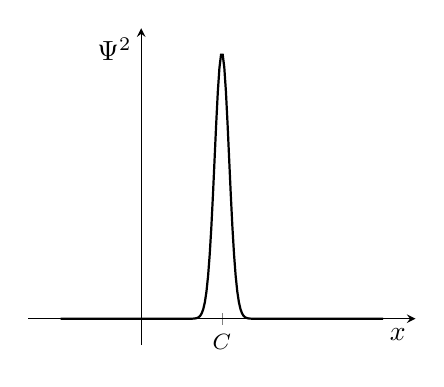
\begin{tikzpicture}
\begin{axis}[small,axis lines=middle,xlabel={$x$},ylabel={$\abs{\Psi}^2$},xtick={0.25},xticklabels={$C$},ytick={\empty},ylabel style={at={(current axis.above origin)},anchor=north east},xlabel style={at={(current axis.right of origin)},anchor=north east},enlargelimits]
\addplot [thick,domain=-0.25:0.75,samples=200,]	{exp(-1000*(x-0.25)^2)};
\end{axis}
\end{tikzpicture}
\caption{
تفاعل موج کا انہدام:  اس لمحے کے فوراً بعد \عددی{\abs{\Psi}^2} کی ترسیم جب پیمائش سے ذرہ  \عددی{C} پر  پایا گیا ہو۔
}
\label{شکل_تفاعل_موج_انہدام}
\end{figure}

%=============================

\حصہ{احتمال} 
\جزوحصہ{ غیر مسلسل متغیرات}\شناخت{جزوحصہ_غیر_مسلسل_متغیرات}
چونکہ کوانٹم میکانیات کی شماریاتی تشریح کی جاتی ہے  لہٰذا  اس میں احتمال کلیدی کردار ادا کرتا ہے۔ اسی لیے میں اصل موضوع سے ہٹ کر  نظریہ احتمال پر تبصرہ کرتا ہوں۔ ہمیں چند نئی علامات   اور اصطلاحات سیکھنی  ہوں  گی جنہیں میں ایک سادہ مثال کی مدد سے  واضح کرتا ہوں۔ 

فرض کریں ایک کمرہ   میں \عددی{14}   افراد  موجود ہیں جن  کی  عمریں درج ذیل ہیں۔ 
\begin{center}
\begin{tabular}{r}
\عددی{14}  سال عمر کا ایک فرد، \\
\عددی{15} سال عمر کا ایک فرد، \\
\عددی{16} سال عمر کے تین افراد، \\
    \عددی{22}  سال عمر کے دو  افراد، \\
\عددی{24}  سال عمر کے دو افراد، \\
        \عددی{25}  سال عمر کے پانچ  افراد۔
\end{tabular}
\end{center}
 
اگر  \عددی{ j }  عمر  کے لوگوں کی  تعداد  کو\عددی{ N(j)} لکھا جائے تو یوں لکھا جائے  گا۔
\begin{align*}
N(14) &= 1 \\
N(15) &= 1 \\
N(16) &= 3 \\
N(22) &= 2 \\
N(24) &= 2 \\
N(25) &= 5 \\
\end{align*}
جبکہ، مثال کے طور پر،  \عددی{N(17)} کی قیمت  صفر ہو گی۔کمرے  میں افراد  کی کل تعداد درج ذیل ہو گی۔ 
\begin{align}
N = \sum_{j=0}^{\infty} N(j)
\end{align}

(اس مثال میں، ظاہر ہے کہ،  \عددی{ N=14 } ہو گا۔)  شکل  \حوالہ{شکل_تفاعل_موج_عمر_مستطیل_ترسیم} میں اس مواد کی مستطیلی ترسیم دکھائی  گئی ہے۔ اس تقسیم کے بارے میں  درج ذیل چند ممکنہ سوالات ابھرتے  ہیں۔ 

\begin{figure}
\centering
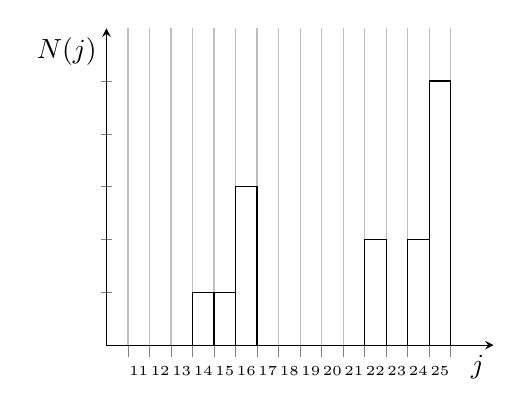
\begin{tikzpicture}
\begin{axis}[small,axis lines=middle,ybar interval,ymin=0,ymax=6,xlabel={$j$},ylabel={$N(j)$},xlabel style={at={(current axis.right of origin)},anchor=north east},ylabel style={at={(current axis.above origin)},anchor=north east},ytick={1,2,3,4,5},yticklabels={},xmax=28,]
\pgfplotsset{every tick label/.append style={font=\tiny}}
\addplot [fill=none]coordinates {(10,0)(11,0)(12,0)(13,0) (14, 1) (15, 1) (16, 3) (17, 0)(18,0)(19,0)(20,0)(21,0) (22, 2) (23, 0) (24,2)(25,5)(26,0) };
\end{axis}
\end{tikzpicture}
\caption{مستطیل ترسیم جس میں عمر \عددی{j} کے لحاظ سے تعداد \عددی{N(j)} دکھائی  گئی ہے۔}
\label{شکل_تفاعل_موج_عمر_مستطیل_ترسیم}
\end{figure}

\ترچھا{سوال 1:}\quad
اگر ہم اس گروہ سے بلا منصوبہ ایک فرد  منتخب کریں تو اس بات کا کیا \اصطلاح{احتمال} ہو گا کہ اس فرد  کی عمر  \عددی{15}   سال ہو؟
\ترچھا{جواب :}\quad
چودہ میں ایک امکان  ہو گا کیونکہ کل  \عددی{14} افراد  ہیں اور ہر ایک فرد کے انتخاب کا امکان ایک جیسا ہے لہٰذا ایسا ہونے کا احتمال چودہ میں سے ایک ہو گا۔  اگر \عددی{j}  عمر کے  فرد کے انتخاب کا احتمال\عددی{ P(j) } ہو تو  \عددی{P(14)=1/14}، \عددی{P(15)=1/14}، \عددی{P(16)=3/14}، وغیرہ ہو گا۔اس کا عمومی کلیہ درج ذیل ہو گا۔
\begin{align}
P(j) = \frac{N(j)}{N} 
\end{align}
دھیان رہے کہ  چودہ یا پندرہ سال عمر کے فرد  کے انتخاب کا احتمال ان دونوں کے  انفرادی احتمال کا مجموعہ یعنی \عددی{ \frac{1}{7} } ہو گا۔واضح رہے کہ  تمام احتمالات کا مجموعہ اکائی \عددی{(1)} کے برابر ہو گا چونکہ آپ کسی نہ کسی عمر کے شخص کو ضرور منتخب کر پائیں گے۔ 
\begin{align}\label{مساوات_تفاعل_موج_کل_احتمال_اکائی}
\sum_{j=0}^{\infty} P(j) = 1
\end{align}

\ترچھا{سوال 2:}\quad
کونسی عمر   \اصطلاح{سب  سے زیادہ  محتمل}\فرہنگ{محتمل!سب سے زیادہ}\حاشیہب{most probable}\فرہنگ{probable!most}  ہے؟
\ترچھا{جواب:} \quad 
\عددی{ 25 }،  چونکہ پانچ اشخاص اتنی عمر رکھتے ہیں جبکہ اس کے بعد ایک جیسی عمر کے لوگوں کی اگلی زیادہ  تعداد تین ہے۔ عمومی طور پر سب سے زیادہ احتمال کا \عددی{j} وہی \عددی{ j } ہو گا جس کے لئے\عددی{ P(j) } کی قیمت زیادہ سے زیادہ ہو۔ 

\ترچھا{سوال 3:} \اصطلاح{وسطانیہ}\فرہنگ{وسطانیہ}\حاشیہب{median}\فرہنگ{median} عمر کیا ہے؟  \ترچھا{جواب:}\quad
چونکہ \عددی{7} لوگوں  کی عمر \عددی{23} سے کم اور \عددی{7} لوگوں  کی  عمر \عددی{23} سے زیادہ ہے۔  لہٰذا  جواب \عددی{ 23 } ہو گا۔ (عمومی طور پر وسطانیہ \عددی{ j } کی وہ قیمت ہو گی جس سے زیادہ  اور جس سے کم قیمت کے نتائج کا احتمال  ایک  جیسا ہو۔)

\ترچھا{سوال 4:}\quad
ان  کی  \اصطلاح{اوسط}\فرہنگ{اوسط}\حاشیہب{mean}\فرہنگ{mean} عمر کتنی ہے ؟\ترچھا{جواب:} 
\begin{align*}
 \frac{(14)+(15)+3(16)+2(22)+2(24)+5(25)}{14} = \frac{294}{14}=21 
\end{align*}
عمومی طور پر \عددی{ j } کی اوسط قیمت جس کو ہم  \عددی{ \langle j \rangle } لکھتے ہیں، درج ذیل ہو گی۔ 
\begin{align}\label{مساوات_تفاعل_موج_اوسط}
\langle j \rangle = \frac{\sum  j N(j)}{N} = \sum_{j=0}^{\infty} jP(j) 
\end{align}
دھیان رہے کہ عین ممکن ہے کہ گروہ میں کسی کی بھی عمر گروہ کی اوسط یا وسطانیہ  کے برابر نہ ہو۔ مثال کے طور پر،  اس مثال میں کسی کی عمر بھی  \عددی{ 21 } یا \عددی{ 23 } سال نہیں ہے۔ کوانٹائی میکانیات میں ہم عموماً اوسط قیمت میں دلچسپی رکھتے ہیں جس کو \اصطلاح{توقعاتی قیمت}\فرہنگ{توقعاتی!قیمت}\حاشیہب{expectation value}\فرہنگ{expectation!value}  کا نام دیا گیا ہے۔ 

\ترچھا{سوال 5:}\quad عمروں کے مربعوں کی  اوسط کیا ہو گی ؟ \ترچھا{جواب:} \quad  آپ \عددی{ \frac{1}{14} } احتمال سے   \عددی{ 14^{2} = 196 }  حاصل کر سکتے ہیں، یا \عددی{ \frac{1}{14} } احتمال سے \عددی{ 15^{2} = 225 }، یا \عددی{ \frac{3}{14} } احتمال سے \عددی{ 16^{2} = 256 } ، وغیرہ  حاصل کر سکتے ہیں۔یوں ان کے مربعوں کی  اوسط درج ذیل ہو گی۔ 
\begin{align}\label{مساوات_تفاعل_موج_اوسط_مربع}
\langle j^{2} \rangle  = \sum_{j=0}^{\infty} j^{2} P(j) 
\end{align}
عمومی طور پر \عددی{ j } کے کسی بھی تفاعل کی اوسط قیمت درج ذیل ہو گی۔ 
\begin{align}
 \langle f(j) \rangle = \sum_{j=0}^{\infty} f(j) P(j) 
\end{align}
(مساوات \حوالہ{مساوات_تفاعل_موج_کل_احتمال_اکائی}، \حوالہ{مساوات_تفاعل_موج_اوسط} اور \حوالہ{مساوات_تفاعل_موج_اوسط_مربع} اس  کی خصوصی صورتیں ہیں۔) یاد  رہے کہ مربع کی  اوسط \عددی{\langle j^2\rangle} عموماً اوسط کے مربع \عددی{\langle j \rangle^2} کے برابر نہیں ہو گی۔ مثال کے طور پر اگر ایک کمرے  میں صرف دو بچے ہوں جن کی عمریں\عددی{ 1 } اور\عددی{ 3 } ہوں  تب 
\عددی{ \langle x^{2} \rangle = 5 } 
 جبکہ
\عددی{ \langle x\rangle ^{2} = 4 } 
 ہو گا۔

\begin{figure}
\centering
\begin{subfigure}{0.45\textwidth}
\centering
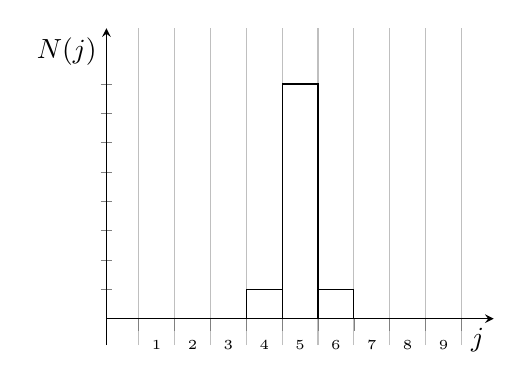
\begin{tikzpicture}
\begin{axis}[small,axis lines=middle,ybar interval,ymin=0,ymax=6,xlabel={$j$},ylabel={$N(j)$},xlabel style={at={(current axis.right of origin)},anchor=north east},ylabel style={at={(current axis.above origin)},anchor=north east},ytick={1,2,3,4,5,6,7,8},yticklabels={},ymax=9,enlargelimits=true]
\pgfplotsset{every tick label/.append style={font=\tiny}}
\addplot[fill=none] coordinates {(1,0)(2,0)(3,0)(4,1)(5,8)(6,1)(7,0)(8,0)(9,0)(10,0) };
\end{axis}
\end{tikzpicture}
\end{subfigure}\hfill
\begin{subfigure}{0.45\textwidth}
\centering
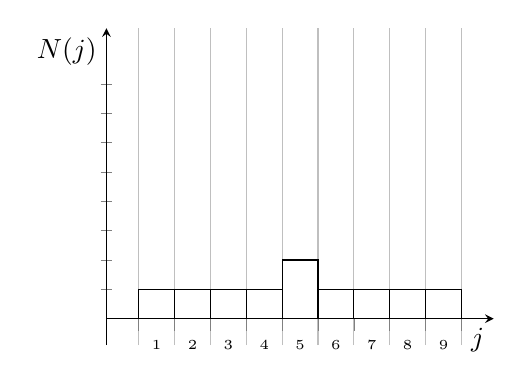
\begin{tikzpicture}
\begin{axis}[small,axis lines=middle,ybar interval,ymin=0,ymax=6,xlabel={$j$},ylabel={$N(j)$},xlabel style={at={(current axis.right of origin)},anchor=north east},ylabel style={at={(current axis.above origin)},anchor=north east},ytick={1,2,3,4,5,6,7,8},yticklabels={},ymax=9,enlargelimits=true]
\pgfplotsset{every tick label/.append style={font=\tiny}}
\addplot[fill=none] coordinates {(1,1)(2,1)(3,1)(4,1)(5,2)(6,1)(7,1)(8,1)(9,1)(10,0) };
\end{axis}
\end{tikzpicture}
\end{subfigure}
\caption{
دونوں مستطیل ترسیمات میں وسطانیہ کی قیمت ایک جیسی ہے، اوسط کی قیمت ایک جیسی ہے  اور سب سے زیادہ  احتمال  کی قیمت ایک جیسی  ہے،   تاہم   ان ترسیمات  میں  معیاری انحراف  مختلف ہیں۔
}
\label{شکل_تفاعل_موج_مختلف_معیاری_انحراف}
\end{figure}

شکل \حوالہ{شکل_تفاعل_موج_مختلف_معیاری_انحراف} کی شکل و صورت  میں واضح فرق پایا جاتا ہے اگرچہ ان کی اوسط کی قیمت ایک جیسی ہے، وسطانیہ کی قیمت  ایک جیسی ہے،  سب سے زیادہ  احتمال کی    قیمت ایک جیسی ہے   اور اجزاء کی تعداد ایک جیسی ہے۔ ان میں پہلی شکل اوسط کے قریب نوکیلے   ابھار جیسی  ہے جبکہ دوسری شکل  افقی چوڑی  صورت رکھتی ہے۔ (مثال کے طور پر کسی بڑے شہر میں ایک جماعت میں طلبہ  کی تعداد پہلی شکل کی   مانند ہو گی جبکہ دیہاتی علاقے    میں ایک ہی کمرے  پر مبنی مکتب  میں بچوں کی تعداد دوسری شکل سے  ظاہر ہو گی۔) ہمیں اوسط قیمت کے لحاظ سے کسی بھی مقدار کی تقسیم کی "وسعت"، عددی صورت میں درکار ہو گی۔ اس کا ایک سیدھا طریقہ یہ ہو سکتا ہے کہ ہم ہر انفرادی جزو کی قیمت اور اوسط قیمت کا فرق
\begin{align}
\Delta j = j-\langle j \rangle 
\end{align}
لے کر  تمام \عددی{ \Delta j } کی اوسط تلاش کریں۔ ایسا کرنے سے یہ مسئلہ پیش آتا ہے کہ ان کا جواب صفر ہو گا چونکہ اوسط کی تعریف کے تحت اوسط سے زیادہ اور اوسط سے کم قیمتیں ایک برابر ہوں گی۔ 
%KKK edited with dr farhan 9 jan 2022
\begin{align*}
\langle \Delta j \rangle &= \sum \left( j -  \langle j \rangle  \right) P(j) = \sum jP(j) - \langle j \rangle \sum P(j) \\
 &= \langle j \rangle - \langle j \rangle = 0
\end{align*}
(چونکہ \عددی{ \langle j \rangle }   مستقل ہے لہٰذا اس کو مجموعہ کی علامت سے باہر لے جایا جا سکتا ہے۔) اس مسئلہ سے چھٹکارا حاصل کرنے کی خاطر  آپ  \عددی{ \Delta j }    کی مطلق قیمتوں کا اوسط لے سکتے ہیں لیکن \عددی{ \Delta j }    کی مطلق قیمتوں  کے ساتھ کام کرنا مشکلات پیدا کرتا ہے۔ اس کی بجائے، منفی علامت سے نجات حاصل کرنے کی خاطر، ہم مربع لینے کے بعد اوسط حاصل کرتے ہیں۔
\begin{align} \label{مساوات_تفاعل_موج_تعریف_معیاری_احتمال_الف}
 \sigma^{2} \equiv \langle \left( \Delta j \right)^{2} \rangle 
\end{align}
اس قیمت کو تقسیم کی \اصطلاح{تغیریت}\فرہنگ{تغیریت}\حاشیہب{variance}\فرہنگ{variance} کہتے ہیں جبکہ تغیریت کا جذر \عددی{ \sigma }  کو \اصطلاح{معیاری انحراف}\فرہنگ{معیاری انحراف}\حاشیہب{standard deviation}\فرہنگ{standard deviation} کہتے ہیں۔ روایتی طور پر  \عددی{\sigma} کو اوسط  \عددی{ \langle j \rangle } کے گرد  وسعت  کی پیمائش  مانا جاتا ہے۔

 ہم تغیریت کا ایک چھوٹا مسئلہ پیش کرتے ہیں۔ 
\begin{align*}
\sigma^{2} &= \langle ( \Delta j )^{2} \rangle = \sum ( \Delta j )^{2} P(j) = \sum (j- \langle j \rangle )^{2} P(j) \\
&= \sum (j^{2} -2j \langle j \rangle + \langle j \rangle ^{2} ) P(j) \\ 
&= \sum j^{2} P(j) -2 \langle j \rangle \sum jP(j) + \langle j \rangle ^{2} \sum P(j) \\ 
&= \langle j^{2}\rangle -2\langle j \rangle \langle j \rangle + \langle j \rangle ^{2} = \langle j^{2} \rangle - \langle j \rangle ^{2}
\end{align*}
اس کا جذر لے کر ہم معیاری انحراف کو درج ذیل لکھ سکتے ہیں۔ 
\begin{align}\label{مساوات_تفاعل_موج_تعریف_معیاری_احتمال_ب}
 \sigma = \sqrt{\langle j^{2} \rangle - \langle j \rangle ^{2}} 
\end{align}


عملی استعمال میں \عددی{ \sigma }  اس کلیے سے بہت جلد حاصل ہو گا۔ آپ \عددی{ \langle j^{2} \rangle } اور \عددی{ \langle j \rangle ^{2} } معلوم کر کہ ان کے فرق کا جذر لیں گے۔ جیسا آپکو یاد ہو گا میں نے ذکر کیا \عددی{ \langle j^{2} \rangle } اور \عددی{ \langle j \rangle ^{2} } عموماً ایک دوسرے کے برابر نہیں ہوں گے۔ جیسا آپ مساوات \حوالہ{مساوات_تفاعل_موج_تعریف_معیاری_احتمال_الف} سے دیکھ سکتے ہیں    \عددی{ \sigma ^{2} } غیر منفی ہو گا لہٰذا  مساوات \حوالہ{مساوات_تفاعل_موج_تعریف_معیاری_احتمال_ب} کے تحت  درج ذیل ہو گا
\begin{align}
 \langle j^2 \rangle \geq \langle j \rangle ^{2}
\end{align}
اور یہ دونوں صرف اس صورت برابر ہو سکتے ہیں جب \عددی{ \sigma = 0 } ہو،   جو تب ممکن ہو گا جب تقسیم میں کوئی  وسعت  نہ پایا جاتا ہو یعنی ہر جزو ایک ہی قیمت کا ہو۔ 


%=========================
\جزوحصہ{استمراری متغیرات}
اب تک ہم غیر مسلسل متغیرات کی بات کرتے آ رہے ہیں  جن کی قیمتیں الگ تھلگ ہوتی ہیں۔ (گزشتہ مثال میں ہم نے افراد کی عمروں کی بات کی جن کو سالوں میں ناپا جاتا ہے  لہٰذا  \عددی{j} عدد صحیح تھا۔)  تاہم اس  کو آسانی سے   استمراری تقسیم  تک وسعت دی جا سکتی ہے۔ اگر میں گلی میں بلا منصوبہ ایک شخص کا انتخاب کر کے اس کی عمر پوچھوں تو اس کا احتمال \ترچھا{صفر} ہو گا کہ اس کی عمر ٹھیک \عددی{16} سال \عددی{4} گھنٹے، \عددی{27} منٹ اور \عددی{3.37524} سیکنڈ ہو۔ یہاں  اس کی عمر کا \عددی{16} اور \عددی{17} سال کے بیچ ہونے کے احتمال کی بات کرنا معقول ہو گا۔بہت کم وقفے کی صورت میں احتمال \ترچھا{وقفے کی لمبائی کے راست متناسب} ہو گا۔ مثال کے طور پر \عددی{16} سال اور \عددی{16} سال جمع دو دنوں کے بیچ عمر  کا احتمال \عددی{16} سال اور \عددی{16} سال جمع ایک دن کے بیچ عمر کے احتمال کا دگنا ہو گا۔(ماسوائے ایسی صورت میں جب  \عددی{16} سال قبل عین اسی دن  کسی وجہ سے بہت زیادہ بچے  پیدا ہوئے ہوں۔ ایسی صورت میں اس قاعدہ کی اطلاق کی نقطہ نظر سے   ایک یا دو دن کا وقفہ بہت لمبا وقفہ ہے۔ اگر زیادہ بچوں کی پیدائش کا دورانیہ چھ گھٹے پر مشتمل ہو تب ہم ایک سیکنڈ یا، زیادہ محفوظ طرف رہنے کی خاطر، اس سے بھی کم دورانیے کا وقفہ لیں گے۔ تکنیکی طور پر ہم لامتناہی چھوٹے وقفہ کی بات کر رہے ہیں۔)  اس طرح درج ذیل لکھا جا سکتا ہے۔
\begin{align}\label{مساوات_تفاعل_موج_وقفہ_پر_احتمال}
 \rho(x)dx =\begin{cases}
\begin{minipage}{0.30\textwidth}
\RL{
بلا منصوبہ منتخب کئے گئے رکن  کا \عددی{x} اور \عددی{(x+\dif x)} کے بیچ پائے جانے کا احتمال
}
\end{minipage}
\end{cases} 
\end{align}
اس مساوات میں تناسبی مستقل \عددی{ \rho(x) } \اصطلاح{کثافت احتمال}\فرہنگ{کثافت!احتمال}\حاشیہب{probability density}\فرہنگ{probability!density} کہلاتا ہے۔  متناہی وقفہ \عددی{a} تا \عددی{b} کے بیچ \عددی{x}  پایا جانے کا احتمال \عددی{ \rho(x) } کا تکمل دے گا:
 \begin{align}
 P_{ab}=\int_a^b \rho(x)\dif x 
 \end{align}
اور غیر مسلسل تقسیم کے لئے اخذ کردہ قواعد درج ذیل روپ اختیار کریں گے:
\begin{align}
1&=\int_{-\infty}^{\infty} \rho(x)\dif x,  \label{مساوات_تفاعل_موج_کل_احتمال_اکائی_ہو_گا}\\
<x>& =\int_{-\infty}^{\infty} x\rho(x)\dif x, \label{مساوات_تفاعل_موج_اوسط_تکمل}\\
\langle f(x)\rangle&=\int_{-\infty}^{+\infty} f(x)\rho(x)\dif x,\\
 \sigma^2&\equiv \langle(\Delta x)^2\rangle = \langle x^2\rangle-\langle x\rangle^2 
\end{align}

\ابتدا{مثال}\شناخت{مثال_تفاعل_موج_چٹان-سے_گرتا_پتھر}
ایک چٹان جس کی اونچائی \عددی{h} ہو سے ایک پتھر کو نیچے گرنے دیا جاتا ہے۔ گرتے ہوئے  پتھر کی بلا واسطہ وقتی فاصلوں پر دس لاکھ تصاویر کھینچے جاتے ہیں۔ ہر تصویر پر طے شدہ فاصلہ ناپا جاتا ہے۔ ان تمام فاصلوں کی\ترچھا{ اوسط} قیمت کیا ہو گی؟ یعنی طے شدہ فاصلوں کا\ترچھا{ وقتی اوسط} کیا ہو گا؟\حاشیہد{ایک ماہر شماریات کو شکوہ ہو گا کہ میں متناہی  نمونہ  (جو یہاں دس لاکھ ہے)  کی اوسط اور (پوری   استمراریہ) پر  "اصلی"  اوسط  میں فرق نہیں کر  پا  رہا ہوں۔ یہ ایک تجربہ کرنے والے کے لئے مصیبت پیدا کر سکتی ہے، خاص کر جب نمونی جسامت  چھوٹی  ہو، تاہم یہاں مجھے صرف اصل اوسط سے غرض ہے، اور  نمونی اوسط اس کی  اچھی تخمین  ہے۔} 

حل: \quad
پتھر ساکن حال سے بتدریج بڑھتی ہوئی رفتار سے نیچے گرتا ہے۔ یہ چٹان کے  بالائی سر کے قریب زیادہ وقت گزارتا ہے لہٰذا  ہم توقع کرتے ہیں کہ
 فاصلہ \عددی{\frac{h}{2}} سے کم ہو گا۔ ہوائی رگڑ کو نظر انداز کرتے ہوئے،  لمحہ \عددی{t} پر فاصلہ \عددی{x} درج ذیل ہو گا۔
\begin{align*}
 x(t) = \frac{1}{2} gt^2 
\end{align*}
اس کی سمتی رفتار  \عددی{\tfrac{\dif x}{\dif t}=gt} ہو گی اور پرواز کا  دورانیہ \عددی{T=\sqrt{2h/g}} ہو گا۔ وقفہ  \عددی{\dif t} میں تصویر کھینچنے کا احتمال \عددی{\tfrac{\dif t}{T}} ہو گا۔ یوں اس کا احتمال کہ ایک تصویر  مطابقتی سعت \عددی{\dif x} میں فاصلہ دے درج ذیل ہو گا:
 \begin{align*}
 \frac{\dif t}{T} = \frac{\dif x}{gt}\sqrt{\frac{g}{2h}} = \frac{1}{2\sqrt{hx}}\dif x
\end{align*}   
 ظاہر ہے کہ کثافت احتمال  (مساوات \حوالہ{مساوات_تفاعل_موج_وقفہ_پر_احتمال}) درج ذیل ہو گا۔
 \begin{align*}
 \rho(x)&=\frac{1}{2\sqrt{hx}} && (0\leq x\leq h)
 \end{align*}
 (اس وقفہ کے باہر کثافت  احتمال صفر ہو گا۔) 

ہم مساوات \حوالہ{مساوات_تفاعل_موج_کل_احتمال_اکائی_ہو_گا} استعمال کر کے اس نتیجہ کی تصدیق کر سکتے ہیں۔
 \begin{align*}
 \int_0^h \frac{1}{2\sqrt{hx}}\dif x = \frac{1}{2\sqrt{h}}\left .(2x^{\frac{1}{2}})\right\vert_0^h =1
 \end{align*}
 مساوات \حوالہ{مساوات_تفاعل_موج_اوسط_تکمل} سے اوسط فاصلہ تلاش  کرتے ہیں
 \begin{align*}
 \langle x\rangle =\int_0^h x\frac{1}{2\sqrt{hx}}\dif x= \frac{1}{2\sqrt{h}} \left . \big(\frac{2}{3}x^{\frac{3}{2}}\big)\right\vert_0^h = \frac{h}{3}
 \end{align*}
 جو  \عددی{ \frac{h}{2}}   سے کچھ کم ہے  جیسا کہ ہم توقع کرتے ہیں۔

\begin{figure}
\centering
\begin{tikzpicture}[declare function={f(\x)=1/(2*sqrt(\x));}]
\begin{axis}[small,axis lines=middle,xlabel={$x$},ylabel={$\rho(x)$},xlabel style={at={(current axis.right of origin)},anchor=north east},ylabel style={at={(current axis.above origin)},anchor=north east},xtick={1},xticklabels={$h$},ytick={0.5},yticklabels={$\tfrac{1}{2h}$},xmin=0,ymin=0,xmax=1.25]
\addplot[domain=0.1:1,smooth,thick] {f(x)};
\addplot[dashed] plot coordinates {(0,0.5)(1,0.5)};
\end{axis}
\end{tikzpicture}
\caption{کثافت احتمال برائے مثال \حوالہ{مثال_تفاعل_موج_چٹان-سے_گرتا_پتھر}: \عددی{\rho(x)=1/(2\sqrt{hx})}}
\label{شکل_تفاعل_موج_کثافت_احتمال_برائے_مثال}
\end{figure}


 شکل  \حوالہ{شکل_تفاعل_موج_کثافت_احتمال_برائے_مثال}  میں   \عددی{ \rho(x)} کی ترسیم دکھائی گئی ہے۔آپ دیکھ سکتے ہیں کہ کثافت احتمال خود لامتناہی ہو سکتا ہے جبکہ  احتمال (یعنی \عددی{\rho} کا تکمل) لازماً  متناہی (بلکہ  \عددی{1} یا \عددی{1} سے کم ہو گا)۔
\انتہا{مثال}
%===================
\ابتدا{سوال}
 حصہ \حوالہ{جزوحصہ_غیر_مسلسل_متغیرات} میں اشخاص کی عمروں کی تقسیم کے لیے درج ذیل کریں۔ 
\begin{enumerate}[a.]
\item
اوسط کا مربع \عددی{\langle i\rangle^2} اور مربع کا اوسط \عددی{\langle j^2\rangle} تلاش کریں۔ 
\item
 ہر \عددی{j}  کے لیے \عددی{\Delta j} دریافت کریں اور مساوات \حوالہ{مساوات_تفاعل_موج_تعریف_معیاری_احتمال_الف} استعمال کرتے ہوئے  معیاری انحراف دریافت کریں۔
\item
 جزو ا اور ب کے نتائج استعمال کرتے ہوئے مساوات  \حوالہ{مساوات_تفاعل_موج_تعریف_معیاری_احتمال_ب} کی تصدیق کریں۔ 
\end{enumerate}
\انتہا{سوال}
%==================
\ابتدا{سوال}
\begin{enumerate}[a.]
\item
 مثال \حوالہ{مثال_تفاعل_موج_چٹان-سے_گرتا_پتھر} کی تقسیم کے لیے معیاری انحراف تلاش کریں۔
\item
بلا واسطہ منتخب تصویر میں  اوسط فاصلے سے، ایک معیاری انحراف کے برابر، دور فاصلہ \عددی{x} پائے جانے کا احتمال کیا ہو گا؟
\end{enumerate}
\انتہا{سوال}
%==================
\ابتدا{سوال}
درج ذیل گاوسی تقسیم پر غور کریں  جہاں    \عددی{A}، \عددی{a} اور \عددی{\lambda} مستقل ہیں۔  
\begin{align*}
\rho(x)=Ae^{-\lambda(x-a)^2}
\end{align*}
   (ضرورت کے پیش آپ تکمل کسی جدول سے دیکھ سکتے ہیں۔)
\begin{enumerate}[a.]
\item
مساوات\حوالہ{مساوات_تفاعل_موج_کل_احتمال_اکائی_ہو_گا} استعمال کرتے ہوئے  \عددی{A} کی قیمت تعین کریں۔
\item
اوسط \عددی{\langle x \rangle}، مربعی اوسط \عددی{\langle x^2\rangle} اور معیاری انحراف \عددی{\sigma} تلاش کریں۔
\item
\عددی{\rho(x)} کی ترسیم کا خاکہ بنائیں۔
\end{enumerate}
\انتہا{سوال}

%====================================
% section 1.4 
\حصہ{معمول زنی}
ہم تفاعل موج کے شماریاتی مفہوم ( مساوات \حوالہ{مساوات_تفاعل_موج_شماریاتی_مفہوم_الف}) پر دوبارہ غور کرتے ہیں، جس کے تحت لمحہ \عددی{t}  پر ایک ذرے کا نقطہ \عددی{x} پر پائے جانے کی کثافت احتمال \عددی{\abs{\Psi(x,t)}^2} ہو گی۔  یوں  
(مساوات \حوالہ{مساوات_تفاعل_موج_کل_احتمال_اکائی_ہو_گا}) کے تحت \عددی{\abs{\Psi}^2} کا تکمل \عددی{1} کے برابر ہو گا (چونکہ ذرہ کہیں نہ کہیں تو ضرور پایا جائے گا)۔ 
\begin{align}\label{مساوات_تفاعل_موج_احتمال_اکائی}
\int_{-\infty}^{+\infty}\abs{\Psi(x,t)}^2 = 1
\end{align}
اس حقیقت کے بغیر شماریاتی مفہوم بے معنی ہو گی۔ 

البتہ یہ شرط آپ کے لیے  پریشانی کا سبب ہونا چاہیے۔   تفاعل موج کو مساوات شروڈنگر تعین کرتی ہے اور \عددی{\Psi} پر بیرونی شرائط مسلط کرنا صرف اس صورت جائز ہو گا جب ان دونوں کے بیچ اختلاف نہ پایا جاتا ہو۔ مساوات \حوالہ{مساوات_تفاعل_موج_شروڈنگر_الف} پر نظر ڈالنے سے آپ دیکھ سکتے ہیں کہ اگر  \عددی{ \Psi (x , t) } حل ہو تب \عددی{ A \Psi (x , t ) } بھی حل ہو گا، جہاں \عددی{A} کوئی بھی (مخلوط) مستقل ہو سکتا ہے۔ اس طرح ہم یہ کر سکتے ہیں کہ نا معلوم  ضربی مستقل کو یوں منتخب کریں کہ  مساوات  \حوالہ{مساوات_تفاعل_موج_احتمال_اکائی} مطمئن ہو۔  اس عمل کو تفاعل موج کی \اصطلاح{معمول زنی}\فرہنگ{معمول زنی}\حاشیہب{normalization}\فرہنگ{normalization} کہتے ہیں۔ہم کہتے ہیں کہ تفاعل موج کو معمول پر لایا گیا ہے۔ مساوات شروڈنگر کے بعض حلوں کا تکمل \ترچھا{لامتناہی} ہو گا؛ ایسی صورت میں کوئی  بھی ضربی مستقل اس کو \عددی{1} کے برابر نہیں کر سکتا ہے۔ یہی کچھ غیر اہم حل \عددی{ \Psi = 0 } کے لیے بھی درست ہے۔ ایسا تفاعل موج جو معمول پر لانے کے قابل نہ ہو  کسی صورت ایک ذرے کو ظاہر نہیں کر سکتا ہے لہٰذا اس کو رد کیا جاتا ہے۔  طبیعی طور پر پائے جانے والے حالات، شروڈنگر مساوات کے  \اصطلاح{مربع متکامل}\فرہنگ{مربع متکامل}\حاشیہب{square-integrable}\فرہنگ{square-integrable}  حل ہونگے۔\حاشیہد{ظاہر ہے کہ \عددی{\abs{x}\to\infty} کی صورت میں \عددی{\Psi(x,t)} کو \عددی{1/\sqrt{\abs{x}}} سے زیادہ تیز صفر تک پہنچنا ہو گا۔ معمول زنی صرف مخلوط عدد کے معیار کو درست کرتی ہے جبکہ اس کا ہیّت غیر معین رہتا ہے۔تاہم جیسا ہم جلد دیکھیں گے، موخر الذکر کی کوئی طبیعی اہمیت نہیں پائی جاتی ہے۔}

 یہاں رک کر ذرا غور کریں!  فرض کریں لمحہ \عددی{ t = 0 } پر میں ایک تفاعل موج کو معمول پر لاتا ہوں۔ کیا وقت گزرنے کے ساتھ \عددی{\Psi} ارتقا پانے کے بعد بھی یہ معمول شدہ رہے گی؟ (آپ ایسا نہیں کر سکتے ہیں  کہ لمحہ در لمحہ  تفاعل موج کو معمول پر لائیں چونکہ ایسی صورت میں \عددی{A} وقت \عددی{t} کا تابع تفاعل ہو گا نا کہ ایک مستقل، اور \عددی{A\Psi} شروڈنگر مساوات کا حل نہیں رہے گا۔) خوش قسمتی سے مساوات شروڈنگر کی یہ ایک خاصیت ہے کہ یہ تفاعل موج  کی معمول شدہ صورت برقرار رکھتی ہے۔ اس خاصیت کے بغیر مساوات شروڈنگر  اور شماریاتی مفہوم غیر ہم آہنگ ہونگے اور  کوانٹم نظریہ بے معنی ہو گا۔

 یہ ایک اہم نقطہ ہے لہٰذا ہم اس کے ثبوت کو غور سے دیکھتے ہیں۔ ہم درج ذیل مساوات سے شروع کرتے ہیں۔
\begin{align}\label{مساوات_تفاعل_موج_الف}
\frac{\dif}{\dif t} \int_{-\infty}^{\infty} \abs{ \Psi (x , t)}^2 \dif x = \int_{- \infty}^{\infty} \frac{ \partial}{\partial t} \abs{ \Psi (x , t)}^2 \dif x 
\end{align}
(دھیان رہے  کہ، مساوات کے بائیں ہاتھ، تکمل صرف \عددی{t}  کا تفاعل ہے لہٰذا میں نے پہلے فقرہ میں کل تفرق \عددی{ \frac{\dif }{\dif t} } استعمال کیا ہے، جبکہ دائیں ہاتھ متکمل \عددی{t} اور \عددی{x} دونوں کا تفاعل ہے لہٰذا میں نے یہاں جزوی تفرق \عددی{\partial/\partial t} استعمال کیا ہے۔  اصول ضرب کے تحت درج ذیل ہو گا۔
\begin{align}
\frac{\partial}{\partial t}\abs{\Psi}=\frac{\partial}{\partial t}(\Psi^*\Psi)=\Psi^*\frac{\partial \Psi}{\partial t}+\frac{\partial \Psi^*}{\partial t}\Psi
\end{align}
اب مساوات شروڈنگر کہتی ہے کہ 
\begin{align}\label{مساوات_تفاعل_موج_شروڈنگر_تفرق_الف}
\frac{\partial \Psi}{\partial t}=\frac{i\hslash}{2m}\frac{\partial^{\,2}\Psi}{\partial x^2}-\frac{i}{\hslash}V\Psi
\end{align}
ہو گا اور ساتھ ہی  (مساوات \حوالہ{مساوات_تفاعل_موج_شروڈنگر_تفرق_الف} کا مخلوط جوڑی دار لیتے ہوئے) 
\begin{align}\label{مساوات_تفاعل_موج_آخر}
\frac{\partial \Psi^*}{\partial t}=-\frac{i\hslash}{2m}\frac{\partial^{\,2}\Psi^*}{\partial x^2}+\frac{i}{\hslash}V\Psi^*
\end{align}
ہو گا لہٰذا درج ذیل لکھا جا سکتا ہے۔
\begin{align}\label{مساوات_تفاعل_موج_صریحاً_تکمل_الف}
\frac{\partial}{\partial t}\abs{\Psi}^2=\frac{i\hslash}{2m}\big(\Psi^*\frac{\partial^{\,2} \Psi}{\partial x^2}-\frac{\partial^{\,2}\Psi^*}{\partial x^2}\Psi^2\big)=\frac{\partial}{\partial x}\big[\frac{i\hslash}{2m}\big(\Psi^*\frac{\partial \Psi}{\partial x}-\frac{\partial \Psi^*}{\partial x}\Psi\big)\big]
\end{align}
مساوات \حوالہ{مساوات_تفاعل_موج_الف} میں تکمل کی قیمت اب  صریحاً معلوم کی جا سکتی ہے:
\begin{align}
\frac{\dif}{\dif t}\int_{-\infty}^{\infty}\abs{\Psi(x,t)}^2\dif x=\left .\frac{i\hslash}{2m}\big(\Psi^*\frac{\partial \Psi}{\partial x}-\frac{\partial \Psi^*}{\partial x}\Psi\big)\right\vert_{-\infty}^{+\infty}
\end{align}
یاد رہے کہ معمول پر لانے کے قابل ہونے کے لئے ضروری ہے کہ \عددی{x\to\pm\infty} کرتے ہوئے \عددی{\Psi(x,t)} صفر\حاشیہد{ایک اچھا ریاضی دان آپ کو بہت سی گھمبیر مثالیں پیش کر سکتا ہے، تاہم  طبیعیات کی میدان  میں ایسے تفاعلات نہیں پائے جاتے ہیں؛ اور  لامتناہی پر تفاعلات موج ہر صورت صفر کو پہنچتے ہیں۔} کو پہنچتی ہو۔یوں درج ذیل ہو گا
\begin{align}\label{مساوات_تفاعل_موج_تکمل_مستقل_ہو_گا}
\frac{\dif}{\dif t}\int_{-\infty}^{\infty}\abs{\Psi(x,t)}^2\dif x=0
\end{align}
لہٰذا تکمل (وقت کا غیر تابع) مستقل ہو گا؛ لمحہ \عددی{t=0} پر معمول شدہ تفاعل موج ہمیشہ کے لئے معمول شدہ رہے گا۔

\ابتدا{سوال}
لمحہ \عددی{t=0} پر ایک ذرہ کو درج ذیل تفاعل موج ظاہر کرتی ہے جہاں \عددی{A}، \عددی{a} اور \عددی{b} مستقلات ہیں۔
\begin{align*}
\Psi(x,0)=
\begin{cases}
A\frac{x}{a}&0\le x\le a\\begin{align*}
0.25em]
A\frac{(b-x)}{(b-a)}&a\le x\le b\\begin{align*}
0.25em]
0&\text{\RL{دیگر صورت}}
\end{cases}
\end{align*}
\begin{enumerate}[a.]
\item
تفاعل موج \عددی{\Psi} کو معمول پر لائیں (یعنی \عددی{a} اور \عددی{b} کی صورت میں \عددی{A} تلاش کریں)۔
\item
متغیر \عددی{x} کے لحاظ سے \عددی{\Psi(x,0)} ترسیم کریں۔
\item
لمحہ \عددی{t=0} پر کس نقطہ پر ذرہ پایا جانے کا احتمال زیادہ سے زیادہ ہو گا؟ 
\item
نقطہ \عددی{a} کے بائیں جانب ذرہ پایا جانے کا احتمال کتنا ہے؟ اپنے جواب کی تصدیق  \عددی{b=a}  اور \عددی{b=2a} کی تحدیدی صورتوں میں کریں۔
\item
متغیر \عددی{x} کی توقعاتی قیمت کیا ہو گی؟
\end{enumerate}
\انتہا{سوال} 
%================

\ابتدا{سوال}
درج ذیل تفاعل موج پر غور کریں جہاں \عددی{A}، \عددی{\lambda} اور \عددی{\omega} مثبت حقیقی مستقلات ہیں۔
\begin{align*}
\Psi(x,t)=Ae^{-\lambda\abs{x}}e^{-i\omega t}
\end{align*}
(ہم باب \حوالہ{باب_غیر_تابع_وقت_شروڈنگر_مساوات} میں دیکھیں گے کہ کس طرح کا \اصطلاح{مخفیہ}\فرہنگ{مخفیہ}\حاشیہب{potential}\فرہنگ{potential} \عددی{V} ایسا تفاعل موج پیدا کرتا ہے۔)
\begin{enumerate}[a.]
\item
تفاعل موج \عددی{\Psi} کو معمول پر لائیں۔
\item
متغیرات \عددی{x} اور \عددی{x^2} کی توقعاتی قیمتیں تلاش کریں۔
\item
متغیر \عددی{x} کا معیاری انحراف تلاش کریں۔ متغیر \عددی{x} کے لحاظ سے \عددی{\abs{\Psi}^2} ترسیم کر کے اس پر  نقاط \عددی{(\langle x\rangle+\sigma)} اور  \عددی{(\langle x\rangle-\sigma)} کی نشاندہی کریں جس سے \عددی{x} کی "پھیل" کو \عددی{\sigma} سے ظاہر کرنے  کی وضاحت ہو گی۔ اس سعت سے باہر ذرہ پایا جانے کا احتمال کتنا ہو گا؟
\end{enumerate}
\انتہا{سوال}
%=============================
\حصہ{معیار حرکت}
 حال \عددی{\Psi} میں پائے جانے والے ذرہ  کے مقام \عددی{x} کی توقعاتی قیمت درج ذیل ہو گی۔
\begin{align}\label{مساوات_تفاعل_موج_معیار_حرکت_توقعاتی_قیمت_تعریف}
\langle x\rangle=\int_{-\infty}^{+\infty}x|\Psi (x,t)|^{2}\dif{x}
\end{align}
اس کا مطلب کیا ہے؟ اس کا  ہرگز یہ مطلب نہیں ہے کہ اگر آپ ایک ہی ذرے کا مقام جاننے کے لیے بار بار پیمائش کریں تو آپ کو نتائج کی اوسط قیمت  \عددی{\int x|\Psi|^{2}\dif{x}} حاصل ہو گی۔ اس کے برعکس: پہلی پیمائش (جس کا نتیجہ غیر متعیین ہے) تفاعل موج کو اس قیمت پر بیٹھنے پر مجبور کرے گا جو پیمائش سے حاصل ہوئی ہو، اس کے بعد (اگر جلد) دوسری پیمائش کی جائے تو وہی نتیجہ دوبارہ حاصل ہو گا۔ حقیقت میں 
\عددی{\langle x\rangle} ان ذرات کی  پیمائشوں کی اوسط ہو گی جو یکساں حال \عددی{\Psi} میں پائے جاتے ہوں۔ یوں یا تو آپ ہر پیمائش کے بعد کسی طرح اس ذرہ کو دوبارہ ابتدائی حال \عددی{\Psi} میں لائیں گے اور یا آپ متعدد ذرات کی \اصطلاح{سگرا}\فرہنگ{سگرا}\حاشیہب{ensemble}\فرہنگ{ensemble} کو ایک ہی حال \عددی{\Psi}  میں لا کر تمام کے مقام کی  پیمائش کریں گے۔ ان نتائج کا اوسط \عددی{\langle x\rangle} ہو گا۔ (میں اس کی تصوراتی شکل یوں پیش کرتا ہوں کہ ایک الماری میں  قطار پر شیشہ کی بوتلیں کھڑی ہیں اور ہر بوتل میں ایک ذرہ پایا جاتا ہے۔ تمام ذرات ایک جیسے  (بوتل کے وسط کے لحاظ سے) حال \عددی{\Psi} میں پائے جاتے ہیں۔ ہر بوتل کے قریب ایک طالب علم  کھڑا ہے جس کے ہاتھ میں ایک فیتا  ہے۔ جب اشارہ  دیا جائے تو تمام طلبہ اپنے اپنے ذرہ  کا مقام ناپتے ہیں۔ ان نتائج کا مستطیلی ترسیم تقریباً \عددی{|\Psi|^2} دیگا جبکہ ان کی اوسط قیمت تقریباً \عددی{\langle x \rangle} ہو گی۔ (چونکہ ہم متناہی تعداد کے ذرات پر تجربہ  کر رہے ہیں لہٰذا  یہ توقع نہیں کیا جا سکتا ہے کہ جوابات بالکل حاصل ہوں گے لیکن بوتلوں  کی تعداد بڑھانے سے نتائج نظریاتی جوابات کے  زیادہ قریب حاصل ہوں گے۔)) مختصراً توقعاتی قیمت ذرات کے  سگرا پر کیے جانے والے تجربات کی اوسط قیمت ہو گی نہ کہ کسی ایک ذرہ پر بار بار تجربات کی نتائج کی اوسط قیمت۔

 چونکہ \عددی{\Psi} وقت اور مقام کا تابع ہے لہٰذا وقت گزرنے کا ساتھ ساتھ \عددی{\langle x\rangle} تبدیل ہو گا۔ ہمیں اس کی سمتی رفتار جاننے میں دلچسپی ہو سکتی ہے۔ مساوات \حوالہ{مساوات_تفاعل_موج_صریحاً_تکمل_الف}  اور \حوالہ{مساوات_تفاعل_موج_معیار_حرکت_توقعاتی_قیمت_تعریف}  سے درج ذیل\حاشیہد{چیزوں کو  صاف صاف رکھنے کی خاطر میں تکمل کے حد نہیں لکھ رہا ہوں۔}  لکھا جا سکتا ہے۔
\begin{align}\label{مساوات_تفاعل_موج_رفتار_توقعاتی_الف}
\frac{\dif \,\langle x \rangle}{\dif{t}}=\int x\frac{\partial}{\partial{t}}|\Psi|^{2}\dif{x}=\frac{i\hslash}{2m}\int x\frac{\partial}{\partial{x}}\big (\Psi ^*\frac{\partial{\Psi}}{\partial{x}}-\frac{\partial{\Psi^ *}}{\partial{x}}\Psi \big)\dif{x}
\end{align}

تکمل بالحصص\حاشیہد{قاعدہ ضرب کے تحت
\begin{align*}
\frac{\dif}{\dif x}(fg)=f\frac{\dif g}{\dif x}+\frac{\dif f}{\dif x}g
\end{align*}
ہو گا جس سے درج ذیل حاصل ہوتا ہے۔ 
\begin{align*}
\int_a^bf\frac{\dif g}{\dif x}\dif x=-\int_a^b\frac{\dif f}{\dif x}g\dif x+\left.fg\right\vert_a^b
\end{align*}
یوں تکمل کی علامت کے اندر ، آپ  حاصل ضرب میں  کسی ایک جزو سے  تفرق اتار کر  دوسرے کے ساتھ چسپاں کر سکتے ہیں؛ اس کی قیمت  منفی علامت اور اضافی سرحدی جزو کی صورت میں آپ کو ادا کرنی ہو  گی۔}  کی مدد سے اس فقرے کی سادہ  صورت حاصل کرتے ہیں۔
\begin{align}
\frac{\dif\, \langle x \rangle}{\dif{t}}=-\frac{i\hslash}{2m}\int\big (\Psi^*\frac{\partial{\Psi}}{\partial{x}}-\frac{\partial{\Psi^*}}{\partial{x}}\Psi \big)\dif{x}
\end{align}
(میں نے یہاں \عددی{\tfrac{\partial{x}}{\partial{x}}=1} استعمال کیا اور سرحدی جزو کو اس بنا پر رد کیا کہ \عددی{(\pm)} لامتناہی پر \عددی{\Psi} کی قیمت  \عددی{0} ہو گی۔ دوسرے جزو پر  دوبارہ تکمل بالحصص لاگو کرتے ہیں۔
\begin{align}\label{مساوات_تفاعل_موج_توقعاتی_قیمت_رفتار}
\frac{\dif \,\langle x \rangle}{\dif{t}}=-\frac{i\hslash}{m}\int\Psi^*\frac{\partial{\Psi}}{\partial{x}} \dif{x}
\end{align}

اس نتیجے سے ہم کیا مطلب حاصل کر سکتے ہیں؟ یہ  \عددی{x} کی توقعاتی قیمت کی سمتی رفتار ہے نا کہ  ذرہ کی سمتی رفتار۔  ابھی تک ہم جو کچھ دیکھ چکے ہیں اس سے ذرہ  کی سمتی رفتار دریافت نہیں کی جا سکتی ہے۔ کوانٹم میکانیات میں ذرہ  کی  سمتی رفتار کا مفہوم واضح  نہیں ہے۔ اگر پیمائش سے قبل ایک ذرے کا مقام  غیر تعیین  ہو تب اس کی سمتی رفتار بھی غیر تعیین ہو گی۔ ہم ایک مخصوص قیمت کا نتیجہ حاصل کرنے کے احتمال کی صرف بات کر سکتے ہیں۔ ہم \عددی{\Psi} جانتے ہوئے کثافت احتمال کی بناوٹ کرنا باب \حوالہ{باب_قواعد_و_ضوابط} میں دیکھیں گے۔ اب کے لیے صرف اتنا جاننا کافی ہے کہ  \ترچھا{سمتی رفتار کی توقعاتی قیمت ذرہ کے مقام کی توقعاتی قیمت کا تفرق ہو گا}۔
\begin{align}\label{مساوات_تفاعل_موج_تعریف_رفتار}
\langle v \rangle=\frac{\dif\langle x \rangle}{\dif{t}}
\end{align}
مساوات \حوالہ{مساوات_تفاعل_موج_توقعاتی_قیمت_رفتار} ہمیں \عددی{\Psi} سے بلا واسطہ \عددی{\langle v\rangle} دیتی ہے۔ 

روایتی طور پر ہم سمتی رفتار کی بجائے  \اصطلاح{معیار حرکت}\فرہنگ{معیار حرکت}\حاشیہب{momentum}\فرہنگ{momentum} \عددی{p=mv} کے ساتھ کام کرتے ہیں۔
\begin{align}\label{مساوات_تفاعل_موج_تعریف_معیار_حرکت}
\langle p \rangle=m\frac{d\langle x \rangle}{\dif{t}}=-i\hslash\int\big (\Psi^*\frac{\partial{\Psi}}{\partial{x}} \big)\dif{x}
\end{align}
میں \عددی{\langle x\rangle} اور \عددی{\langle p \rangle} کو زیادہ معنی خیز طرز میں پیش کرتا ہوں۔
\begin{align}
\langle x \rangle &=\int \Psi^*(x)\Psi \dif{x}\label{مساوات_تفاعل_موج_توقعاتی_مقام}\\
\langle p \rangle&=\int \Psi^*\big (\frac{\hslash}{i}\frac{\partial}{\partial{x}}\big )\Psi \dif{x}\label{مساوات_تفاعل_موج_توقعاتی_معیار_حرکت}
\end{align}
کوانٹم میکانیات میں  مقام کو \اصطلاح{عامل}\فرہنگ{عامل}\حاشیہب{operator}\فرہنگ{operator} \عددی{x} "ظاہر" کرتا ہے  اور معیار حرکت
 کو عامل \عددی{\frac{\hslash}{i}\frac{\partial }{\partial{x}}} "ظاہر" کرتا\حاشیہد{ایک "عامل" آپ کو  ہدایت  دیتی ہے  کہ عامل کے بعد آنے والے تفاعل کے ساتھ آپ کو  \ترچھا{کیا کرنا}   ہو گا۔ عامل\شناخت{حاشیہ_تفاعل_موج_عاملین_تبصرہ} مقام آپ سے کہتا ہے کہ آپ \عددی{x} سے ضرب دیں۔ عامل معیار حرکت کہتا ہے کہ \عددی{x} کے لحاظ سے تفرق لیں (اور  نتیجہ کو \عددی{-i\hslash} سے ضرب دیں)۔ اس کتاب میں تمام عاملین    تفرقات (\عددی{\dif/\dif t}، \عددی{\dif^{\,2}/\dif t^2}، \عددی{\partial^{\,2}/\partial x\partial y}، وغیرہ) یا ضرب کار (\عددی{2}، \عددی{i}، \عددی{x^2}، وغیرہ)،  اور یا ان دونوں  کے ملاپ ہوں  گے۔}   ہے۔  کسی بھی توقعاتی قیمت کے حصول کی خاطر ہم موزوں عامل کو \عددی{\Psi^*} اور \عددی{\Psi} کے بیچ لکھ کر تکمل لیتے ہیں۔

یہ سب بہت اچھا ہے  لیکن دیگر مقداروں کا کیا ہو گا؟ حقیقت یہ ہے کہ تمام کلاسیکی متغیرات کو مقام اور معیار حرکت کی صورت میں لکھا جا سکتا ہے۔ مثال کے طور پر حرکی توانائی کو
\begin{align*}
T=\frac{1}{2}mv^{2}=\frac{p^{2}}{2m}
\end{align*}
اور زاویائی معیار حرکت کو 
\begin{align*}
\mat{L}=\mat{r}\times m\mat{v}=\mat{r}\times \mat{p}
\end{align*}
لکھا جا سکتا ہے (جہاں یک بعدی حرکت کے لئے  زاویائی معیار حرکت نہیں پایا جاتا ہے)۔ کسی بھی مقدار مثلاً \عددی{Q(x,p)} کی توقعاتی قیمت  حاصل کرنے کے لیے ہم ہر \عددی{p}  کی جگہ \عددی{\tfrac{\hslash}{i}\frac{\dif}{\dif{x}}} پر کر کے حاصل عامل کو \عددی{  \Psi^*} اور \عددی{\Psi} کے بیچ لپیٹ کر درج ذیل تکمل حاصل کرتے ہیں۔
\begin{align}\label{مساوات_تفاعل_موج_توقعاتی_قیمت_حصول}
\langle Q(x,p) \rangle=\int \Psi^*Q\big (x,\frac{\hslash}{i}\frac{\partial}{\partial{x}}\big )\Psi \dif{x}
\end{align}
مثال کے طور پر حرکی توانائی کی توقعاتی قیمت درج ذیل ہو گی۔
\begin{align}
\langle T \rangle=-\frac{\hslash ^{2}}{2m}\int \Psi^*\frac{\partial^{\,2}\Psi}{\partial{x^{2}}}\dif{x}
\end{align}
حال \عددی{\Psi} میں ایک ذرہ کی کسی بھی حرکی مقدار کی توقعاتی قیمت  مساوات \حوالہ{مساوات_تفاعل_موج_توقعاتی_قیمت_حصول}  سے حاصل ہو گی۔
مساوات \حوالہ{مساوات_تفاعل_موج_توقعاتی_مقام} اور \حوالہ{مساوات_تفاعل_موج_توقعاتی_معیار_حرکت}  اس کی دو مخصوص صورتیں ہیں۔ میں نے کوشش کی ہے کہ جناب بوہر کی شماریاتی تشریح کو مد نظر رکھتے ہوئے   مساوات  \حوالہ{مساوات_تفاعل_موج_توقعاتی_قیمت_حصول} قابل قبول نظر آئے، اگرچہ، حقیقتاً یہ کلاسیکی میکانیات سے بہت مختلف انداز ہے کام کرنے کا۔ ہم باب \حوالہ{باب_قواعد_و_ضوابط}  میں اس کو زیادہ مضبوط نظریاتی بنیادوں پر کھڑا کریں گے، جب تک آپ اس کے استعمال  کی مشق کریں۔ فی الحال آپ اس کو ایک مسلمہ تصور کر سکتے ہیں۔

\ابتدا{سوال}
آپ کیوں مساوات \حوالہ{مساوات_تفاعل_موج_رفتار_توقعاتی_الف} کے وسطی فقرہ پر تکمل بالحصص کرتے ہوئے، وقتی تفرق کو \عددی{x} کے اوپر سے گزار کر،یہ جانتے ہوئے کہ \عددی{\tfrac{\partial x}{\partial t}=0} ہے، فیصلہ نہیں کر سکتے ہیں کہ \عددی{\tfrac{\dif  \langle x\rangle}{\dif t}=0} ہو گا؟
\انتہا{سوال}
%=====================  
\ابتدا{سوال}
\عددی{\tfrac{\dif \langle p\rangle}{\dif t}} کا حساب کریں۔\ترچھا{جواب:}
\begin{align}\label{مساوات_تفاعل_موج_مخفی_توانائی_سے_معیار_حرکت}
\frac{\dif\langle p \rangle}{\dif t}=\big\langle-\frac{\partial V}{\partial x} \big\rangle
\end{align}
مساوات \حوالہ{مساوات_تفاعل_موج_تعریف_رفتار} (مساوات \حوالہ{مساوات_تفاعل_موج_تعریف_معیار_حرکت} کا پہلا حصہ) اور \حوالہ{مساوات_تفاعل_موج_مخفی_توانائی_سے_معیار_حرکت} \اصطلاح{مسئلہ اہرنفسٹ}\فرہنگ{مسئلہ!اہرنفسٹ}\حاشیہب{Ehrenfest's theorem}\فرہنگ{theorem!Ehrenfest} کی مخصوص صورتیں ہیں، جو کہتا ہے کہ توقعاتی قیمتیں کلاسیکی قواعد کو مطمئن کرتے ہیں۔
\انتہا{سوال}
%==============
\ابتدا{سوال}
فرض کریں آپ مخفی توانائی کے ساتھ ایک مستقل جمع کرتے ہیں (مستقل سے میرا مراد ایسا مستقل ہے  جو \عددی{x} اور \عددی{t} کا تابع نہ ہو)۔ کلاسیکی میکانیات میں یہ کسی بھی چیز پر اثر انداز نہیں ہو گا البتہ کوانٹم میکانیات میں اس کے اثر پر غور کرنا باقی ہے۔ دکھائیں کہ تفاعل موج کو اب \عددی{e^{-iV_t/\hslash}} ضرب کرتا ہے جو وقت کا تابع جزو ہے۔اس کا کسی حرکی متغیر کی توقعاتی قیمت پر کیا اثر ہو گا؟ 
\انتہا{سوال}
%=========================

\حصہ{اصول عدم یقینیت}\شناخت{حصہ_تفاعل_موج_عدم_یقینیت_اصول}
فرض کریں آپ ایک لمبی رسی کا  بایاں  سر اوپر نیچے  ہلا کر موج پیدا کرتے ہیں (شکل \حوالہ{شکل_تفاعل_موج_مقام_غیر_معین})۔ اب اگر پوچھا جائے کہ یہ موج ٹھیک  کہاں پائی جاتی ہے تو آپ غالباً اس کا جواب دینے سے قاصر ہونگے۔ موج کسی ایک جگہ نہیں بلکہ  \عددی{60}  میٹر لمبائی پر پائی جاتی ہے۔ اس کی بجائے اگر  \اصطلاح{طول موج}\فرہنگ{طول موج}\حاشیہب{wavelength}\فرہنگ{wavelength} پوچھی جائے  تو آپ اس کا معقول جواب دے سکتے ہیں:  اس کا طول موج تقریباً    \عددی{7}  میٹر ہے۔ اس کے برعکس اگر آپ رسی کو ایک جھٹکا دیں تو  ایک نوکیلی موج پیدا ہو گی
 (شکل \حوالہ{شکل_تفاعل_موج_طول_موج_غیر_معین})۔ یہ موج دوری نہیں ہے لہٰذا اس کے طول موج کی بات کرنا بے معنی ہو گا۔ اب آپ طول موج بتانے سے قاصر ہوں گے جبکہ  موج کا مقام بتانا ممکن ہو گا۔ اول الذکر  میں موج کا مقام پوچھنا بے معنی سوال ہو گا جبکہ موخر الذکر میں طول موج جاننا بے معنی  ہو گا۔ ہم ان دو صورتوں کے بیچ کے حالات بھی پیدا کر سکتے ہیں  جن میں  مقام موج   اور  طول موج خاصی حد تک قابل تعین ہوں۔ تاہم ان صورتوں میں طول موج بہتر سے بہتر جانتے ہوئے مقام موج کم سے کم بتانا ممکن ہو گا یا پھر مقام بہتر سے بہتر جانتے ہوئے طول موج کم سے کم قابل تعین   ہو گا۔ فوریئر تجزیہ کا ایک مسئلہ ان حقائق کو مضبوط بنیادوں پر کھڑا کرتا ہے۔ فی الحال میں صرف کیفی دلائل پیش کرنا چاہتا ہوں۔

\begin{figure}
\centering
\begin{minipage}{0.45\textwidth}
\centering
\begin{tikzpicture}[declare function={f(\x)=cos(360/7*\x);g(\x)=e^(-0.1*(\x-14))*cos(360/7*\x);
gg(\x)=e^(0.1*(\x+14))*cos(360/7*\x);h(\x)=-e^(-0.1*(\x-14)-0.3*(\x-17.5))*cos(360/60*(\x-17.5));hh(\x)=-e^(0.1*(\x+14)+0.3*(\x+17.5))*cos(360/50*(\x+17.5));}]
\begin{axis}[clip=false,axis lines=middle,small,xtick={-20,-10,10,20,30},xticklabels={$10$,$20$,$40$,$50$,$60$},ytick={\empty}, y axis line style={draw=none},xmax=35,xlabel={[میٹر]},xlabel style={at={(current axis.right of origin)},anchor={north west}}]
\addplot[thick,domain=-14:14,samples=600]{f(x)};
\addplot[thick,domain=14:17.5,smooth]{g(x)};
\addplot[thick,domain=17.5:35,smooth]{h(x)};
\addplot[thick,domain=-14:-17.5,smooth]{gg(x)};
\addplot[thick,domain=-17.5:-30,smooth]{hh(x)};
\addplot[fill] plot coordinates {(-30,0)}node[circ]{};
\end{axis}
\end{tikzpicture}
\caption{اس موج کا طول موج اچھا خاصا   معین جبکہ مقام غیر معین ہے۔}
\label{شکل_تفاعل_موج_مقام_غیر_معین}
\end{minipage}\hfill
\begin{minipage}{0.45\textwidth}
\centering
\begin{tikzpicture}
\begin{axis}[clip=false,small,axis lines=middle,xlabel={\empty},xtick={\empty},ytick={\empty},ylabel style={at={(current axis.above origin)},anchor=north east},xlabel style={at={(current axis.right of origin)},anchor=north east},y axis line style={draw=none},xtick={-20,-10,10,20,30},xticklabels={$10$,$20$,$40$,$50$,$60$},xmax=35,xlabel={[میٹر]},xlabel style={at={(current axis.right of origin)},anchor={north west}}]
\addplot[smooth,thick] plot coordinates {(-30,0)(-5,0)};
\addplot[smooth,thick] plot coordinates {(5,0)(30,0)};
\addplot[smooth,thick] plot coordinates {(-5,0)(-4,0.2)(0,1)(4,0.2)(5,0)};
\addplot[fill] plot coordinates {(-30,0)}node[circ]{};
\end{axis}
\end{tikzpicture}
\caption{اس موج کا مقام اچھا خاصا  معین جبکہ   طول موج غیر معین ہے۔}
\label{شکل_تفاعل_موج_طول_موج_غیر_معین}
\end{minipage}
\end{figure}

 یہ حقائق ہر موجی مظہر، بشمول کوانٹم میکانی موج تفاعل، کے لیے درست ہیں۔ اب ایک ذرے کے \عددی{\Psi} کے طول موج اور  معیار حرکت کا تعلق  \اصطلاح{کلیہ ڈی بروگ لی}\فرہنگ{کلیہ!ڈی بروگ لی}\حاشیہب{De Broglie formula}\فرہنگ{formula!De Broglie}
\begin{align}\label{مساوات_تفاعل_موج_ڈی_بروگلی_معیار_حرکت}
p=\frac{h}{\lambda}=\frac{2\pi\hslash}{\lambda}
\end{align}
پیش\حاشیہد{میں اس کا ثبوت جلد پیش کروں گا۔ بعض  مصنفین کلیہ ڈی بروگ لی کو ایک مسلمہ  لے کر عامل \عددی{\tfrac{\hslash}{i}\partial/\partial x} سے  معیار حرکت کی شراکت  اخذ کرتے ہیں۔ اگرچہ یہ  تصور زیادہ  خوش اسلوب ہے، تاہم  میں اس راستے پر نہیں چلوں گا چونکہ اس میں پیچیدہ ریاضی درکار ہے جو اصل گفتگو سے دھیان ہٹاتی ہے۔} کرتا ہے۔یوں طول موج میں وسعت  معیار حرکت میں  وسعت  کے مترادف  ہے اور  اب ہمارا عمومی مشاہدہ  یہ  ہو گا کہ کسی ذرے کا مقام ٹھیک ٹھیک جانتے ہوئے ہم اس کی معیار حرکت  کم سے کم  جان سکتے ہیں۔ اس کو ریاضیاتی روپ میں لکھتے ہیں:
\begin{align}\label{مساوات_تفاعل_موج_اصول_عدم_یقینیت}
\sigma_{x}\sigma_{p}\ge\frac{\hslash}{2}
\end{align}
جہاں \عددی{\sigma_x} اور \عددی{\sigma_p} بالترتیب \عددی{x} اور \عددی{p} کے معیاری انحراف ہیں۔ یہ جناب ہیزنبرگ کا مشہور \اصطلاح{اصول عدم یقینیت}\فرہنگ{عدم یقینیت اصول}\فرہنگ{اصول!عدم یقینیت}\حاشیہب{uncertainty principle}\فرہنگ{uncertainty principle}  ہے۔ (اس کا ثبوت  باب \حوالہ{باب_قواعد_و_ضوابط} میں پیش کیا جائے گا۔میں نے اس کو یہاں اس لئے متعارف کیا کہ آپ باب \حوالہ{باب_غیر_تابع_وقت_شروڈنگر_مساوات} کی مثالوں میں اس کا استعمال کرنا سیکھیں۔)

 اس بات کی تسلی کر لیں کہ آپ کو اصول عدم یقینیت کا مطلب سمجھ آ گیا ہے۔  مقام کی پیمائش کی ٹھیک ٹھیک نتائج کی طرح معیار حرکت کی پیمائش بھی ٹھیک ٹھیک نتائج دے گی۔ یہاں  "وسعت" سے مراد یہ ہے کہ یکساں تیار کردہ  نظاموں پر پیمائشیں  بالکل ایک جیسے نتائج  نہیں دیں گی۔  آپ چاہیں تو (\عددی{\Psi} کو نوکیلی بنا کر) ایسا حال تیار کر سکتے ہیں جس پر مقام کی پیمائشیں قریب قریب نتائج  دیں لیکن ایسی صورت میں معیار حرکت کی پیمائشوں کے نتائج ایک دوسرے سے بہت مختلف ہوں گی۔ اس طرح آپ چاہیں تو (\عددی{\Psi} کو ایک لمبی سائن نما موج بنا کر) ایسا حال تیار کر سکتے ہیں جس پر معیار حرکت کی پیمائشوں کے نتائج ایک دوسرے کے قریب قریب ہوں گے لیکن ایسی صورت میں ذرے کے مقام کی پیمائشوں کے نتائج ایک دوسرے سے بہت مختلف ہوں گے۔اور ہاں آپ ایسا حال بھی تیار کر سکتے ہیں جس میں نہ تو مقام  اور نا ہی معیار حرکت ٹھیک سے معلوم ہو۔ مساوات \حوالہ{مساوات_تفاعل_موج_اصول_عدم_یقینیت} درحقیقت ایک عدم مساوات ہے جس میں \عددی{\sigma_x} اور \عددی{\sigma_p} کی جسامت پر کوئی حد مقرر نہیں ہے۔ آپ \عددی{\Psi} کو ایک لمبی بلدار لکیر بنا کر، جس میں بہت سارے ابھار اور گڑھے پائے جاتے ہوں اور جس میں کوئی تواتر نہ پایا جاتا ہو، \عددی{\sigma_x} اور \عددی{\sigma_p} کی قیمتیں جتنی چاہیں بڑھا سکتے ہیں۔
%================

\ابتدا{سوال}\شناخت{سوال_تفاعل_موج_حال_ذرہ}
ایک ذرہ جس کی کمیت \عددی{m} ہے درج ذیل حال میں پایا جاتا ہے 
\begin{align*}
\Psi (x,t)=Ae^{-a[(mx^{2}/\hslash)+it]}
\end{align*}
جہاں \عددی{A} اور \عددی{a} مثبت حقیقی مستقل ہیں۔
\begin{enumerate}[a.]
\item
مستقل \عددی{A} تلاش کریں۔
\item
کس مخفی توانائی تفاعل \عددی{V(x)} کے لیے \عددی{\Psi} شروڈنگر مساوات کو مطمئن کرتا ہے؟
\item
\عددی{x}، \عددی{x^2}، \عددی{p} اور \عددی{p^2} کی توقعاتی قیمتیں تلاش کریں۔
\item
\عددی{\sigma_x} اور \عددی{\sigma_p} کی قیمتیں تلاش کریں۔ کیا ان کا حاصل ضرب اصول عدم یقینیت پر پورا اترتے ہیں؟
\end{enumerate}
\انتہا{سوال}
%====================
\ابتدا{سوال} 
مستقل \عددی{\pi} کے  ہندسی  توسیع  کے اولین \عددی{25} ہندسوں \عددی{(3,1,4,1,5,9,\cdots)}  پر غور کریں۔
\begin{enumerate}[a.]
\item
اس گروہ سے بلا منصوبہ ایک ہندسہ  منتخب کیا جاتا ہے۔ صفر تا نو ہر ہندسہ کے انتخاب کا احتمال کیا ہو گا؟
\item
 کسی ہندسے کے انتخاب کا احتمال سب سے زیادہ ہو گا؟ وسطانیہ ہندسہ کونسا ہو گا؟ اوسط قیمت کیا ہو گی؟
\item
اس تقسیم کا معیاری انحراف کیا ہو گا؟
\end{enumerate}
\انتہا{سوال}
%===========================
\ابتدا{سوال}\شناخت{سوال_تفاعل_موج_سوئی_الف}
گاڑی کی رفتار پیما کی خراب سوئی آزادانہ  طور پر حرکت کرتی ہے۔ ہر جھٹکا کے بعد یہ اطراف سے ٹکڑا کر \عددی{0} اور \عددی{\pi} زاویوں کے بیچ آ کر رک جاتی ہے۔
\begin{enumerate}[a.] 
\item

کثافت احتمال \عددی{\rho(\theta)} کیا ہو گا؟ اشارہ: زاویہ \عددی{\theta} اور \عددی{(\theta+\dif \theta)} کے بیچ سوئی رکنے کا احتمال \عددی{\rho (\theta)\dif\theta} ہو گا۔ متغیر \عددی{\theta} کے لحاظ سے \عددی{\rho(\theta)} کو وقفہ\عددی{-\tfrac{\pi}{2}} تا \عددی{\tfrac{3\pi}{2}} ترسیم کریں (ظاہر ہے اس وقفے کا کچھ حصہ درکار نہیں ہے جہاں \عددی{\rho} صفر ہو گا)۔ دھیان رہے کہ کل احتمال \عددی{1} ہو گا۔
\item
اس تقسیم کے لیے \عددی{\langle \theta \rangle}، \عددی{\langle \theta^2 \rangle} اور \عددی{\sigma} تلاش  کریں۔
\item
 اسی طرح \عددی{\langle \sin\theta \rangle}، \عددی{\langle \cos\theta \rangle} اور \عددی{\langle \cos^2\theta \rangle} تلاش کریں۔
\end{enumerate}
\انتہا{سوال}
%=========================
%the above is edited. what follows till the end of the chapter is not edited


\ابتدا{سوال}\شناخت{سوال_تفاعل_موج_سوئی_ب}
  ہم گزشتہ سوال کے رفتار پیما  کی سوئی پر دوبارہ بات کرتے ہیں  تاہم  اس  مرتبہ  ہم سوئی کے سر کے  \عددی{x} محدد (   یعنی  افقی لکیر پر سوئی کے سایہ ) میں   ہم دلچسپی رکھتے ہیں ۔
\begin{enumerate}[a.]
\item  
   \عددی{\rho(x)} کی کثافت احتمال کیا ہو گی ؟  \عددی{x} کے لحاظ  سے   \عددی{\rho( x )}  کو  \عددی{-2 r} تا  \عددی{+ 2 r}   ترسیم  کریں  جہاں  \عددی{r} سوئی کی لمبائی ہے ۔ تصدیق کر لیں کہ کل  احتمال  \عددی{1} ہے۔  اشارہ :   \عددی{x} اور \عددی{(x + \dif x)}  کے بیچ   \عددی{\psi} کی موجودگی کا  احتمال  \عددی{\rho(x) \dif x} ہے۔ آپ سوال \حوالہ{سوال_تفاعل_موج_سوئی_الف}  سے کسی مخصوص خطہ میں   \عددی{\theta}  کا  احتمال  جانتے ہیں؛  سوال یہ ہے کہ \عددی{\dif  \theta}  کا  مطابقتی  \عددی{\dif x}  کیا ہو گا ؟
\item
   اس تقسیم کے لیے \عددی{\langle x \rangle}،  \عددی{\langle x^2 \rangle} اور  \عددی{\sigma}  تلاش کریں ۔ آپ ان قیمتوں کو سوال \حوالہ{سوال_تفاعل_موج_سوئی_الف} کے جزو (ج) سے کس طرح حاصل کر سکتے ہیں؟
 \end{enumerate}
\انتہا{سوال}
\ابتدا{سوال} 
 ایک کاغذ پر افقی لکیریں کھینچی جاتی ہیں جن کے بیچ فاصلہ  \عددی{L}   رکھا جاتا ہے ۔ کچھ  بلندی سے اس کاغذ پر  \عددی{L} لمبائی کی  ایک سوئی گرائی  جاتی ہے۔  کیا  احتمال  ہو گا کہ یہ  سوئی کسی   لکیر کو کاٹ کر  صفحہ  پر آن ٹہرے ۔ اشارہ : سوال \حوالہ{سوال_تفاعل_موج_سوئی_ب}  سے رجوع کریں ۔ 
\انتہا{سوال}
\ابتدا{سوال}\شناخت{سوال_تفاعل_موج_رو_احتمال}
 لمحہ  \عددی{t} پر  \عددی{( a < x < b )} کے بیچ ایک ذرہ   پایا جانے کا  احتمال  \عددی{P_{ab} (t)} ہے ۔ 
\begin{enumerate}[a.]
\item
 درج ذیل دکھائیں
\begin{align*}
\frac{ \dif P_{ab} }{ \dif t } = J ( a , t ) - J ( b , t )
\end{align*}
جہاں 
\begin{align*}
J( x , t ) =  \frac{ i\hslash}{ 2 m } \big( \Psi \frac{  \partial \Psi^* }{ \partial x } - \Psi^* \frac{ \partial \Psi }{ \partial x } \big)
\end{align*}
ہے۔
\عددی{J ( x , t )} کی اکائی کیا ہو گی ؟   تبصرہ:  چونکہ \عددی{J} آپ کو بتاتا ہے کہ نقطہ \عددی{x}  پر  احتمال  کس رفتار سے گزرتا ہے    لہٰذا   \عددی{J} کو  \اصطلاح{رو احتمال  }\فرہنگ{رو!احتمال}\حاشیہب{probability current}\فرہنگ{probability current}  کہتے ہیں - اگر \عددی{P_{ab} (t)} بڑھ رہا ہو تب  خطہ   کے ایک  سر  میں    احتمال  کے آمد خطہ  کے دوسرے سر سے     احتمال کے نکاس    سے زیادہ ہو گا۔  
\item
 سوال  \حوالہ{سوال_تفاعل_موج_حال_ذرہ}  میں تفاعل موج  کا  احتمال  \عددی{\rho} کیا ہو گا ؟  (یہ زیادہ مزیدار مثال نہیں ہے؛  بہتر مثال جلد پیش کی جائے گی۔)
\end{enumerate}
\انتہا{سوال}
\ابتدا{سوال}
فرض کریں آپ ایک \اصطلاح{غیر مستحکم ذرہ}\فرہنگ{ذرہ!غیر مستحکم}\حاشیہب{unstable particle}\فرہنگ{particle!unstable}   کے بارے میں بات کرنا چاہیں جس کا  خود بخود  ٹکڑے ہونے   کا  "عرصہ حیات''  \عددی{\tau} ہے۔ ایسی صورت میں کہیں پر   ذرہ  پایا جانے کا کل  احتمال  مستقل نہیں بلکہ وقت کے ساتھ (ممکنہ طور پر) قوت نمائی   گھٹے گا۔
ہے۔
\begin{align*}
P(t) = \int_{-\infty }^{ \infty } \abs{\Psi ( x , t )}^2 \dif x=e^{-t/\tau}
\end{align*} 
 اس نتیجے کو    (غیر نفیس طریقہ) سے حاصل کرتے ہیں۔   مساوات  \حوالہ{مساوات_تفاعل_موج_آخر}  میں ہم نے کہے بغیر   فرض کیا کہ مخفی توانائی   \عددی{V}  ایک حقیقی مقدار ہے ۔ یہ ایک معقول بات ہے   تاہم  اس سے مساوات  \حوالہ{مساوات_تفاعل_موج_تکمل_مستقل_ہو_گا}  میں دی گئی   بقا احتمال     پیدا ہوتی ہے۔ آئیں  \عددی{V}   کو مخلوط تصور کر کے دیکھیں۔
\begin{align*}
V = V_0 - i \Gamma
\end{align*}
جہاں  \عددی{V_o} حقیقی مخفی  توانائی   اور  \عددی{\Gamma}  مثبت حقیقی مستقل ہے ۔ 
 \begin{enumerate}[a.]
 \item
 دکھائیں کہ اب (مساوات  \حوالہ{مساوات_تفاعل_موج_تکمل_مستقل_ہو_گا}  کی جگہ)  ہمیں درج ذیل ملتا ہے ۔  
\begin{align*}
\frac{ \dif P }{ \dif t } = -\frac{ 2\Gamma }{\hslash} p
\end{align*}
\item
\عددی{P(t)}  کے لیے حل کریں اور ذرے کا عرصہ حیات    \عددی{\Gamma} کی صورت میں حاصل کریں۔
\end{enumerate}
\انتہا{سوال}
\ابتدا{سوال}
مساوات  شروڈنگر  کے کسی بھی   دو عدد (معمول پر لانے کے قابل)  حل \عددی{\Psi_1}، \عددی{\Psi_2} کے لئے درج ذیل ہو گا۔  
\begin{align*}
\frac{ \dif }{ \dif t } \int_{ - \infty }^{ \infty } \Psi_1^* \Psi_2 \dif x = 0
\end{align*}
\انتہا{سوال}
\ابتدا{سوال}
لمحہ   \عددی{t=0}  پر ایک ذرے کو درج ذیل تفاعل موج   ظاہر کرتا ہے ۔ 
\begin{align*}
\Psi(x,0)=
\begin{cases}
 A( a^2  - x^2 )  & -a \leq x \leq +a \\
0 &\text{\RL{دیگر صورت}}
\end{cases}
\end{align*}
\begin{enumerate}[a.]
\item
معمول زنی مستقل  \عددی{A} تلاش کریں ۔ 
\item
 لمحہ  \عددی{t=0}  پر  \عددی{x}   کی توقعاتی قیمت تلاش کریں ۔
\item
 لمحہ  \عددی{t=0} پر  \عددی{p}  کی توقعاتی قیمت تلاش کریں۔  دھیان رہے  کہ  آپ اس کو  \عددی{ P = m\dif  \langle x \rangle/\dif t }    سے حاصل نہیں کر سکتے ہیں ۔ ایسا کیوں ہے ؟
\item
\عددی{x^2} کی توقعاتی قیمت دریافت کریں۔ 
\item
\عددی{p^2}  کی توقعاتی قیمت دریافت کریں ۔  
\item
\عددی{x ( \sigma_x)}  میں   عدم یقینیت  دریافت کریں ۔ 
\item
\عددی{p ( \sigma_p )} میں عدم یقینیت دریافت کریں ۔
\item
 تصدیق کریں کہ آپ کے نتائج اصول عدم یقینیت  کے عین مطابق ہیں ۔
\end{enumerate}
\انتہا{سوال}
\ابتدا{سوال} 
عمومی طور پر کوانٹم میکانیات اس وقت کارآمد   ہو گی  جب   ذرے  کا  ڈی بروگلی طول موج \عددی{(\hslash/p)}  نظام کی  جسامت \عددی{(d)} سے زیادہ ہو ۔ درجہ    \عددی{T} (کیلون)   پر حراری توازن میں ایک   ذرہ  کی اوسط حرکی توانائی درج ذیل ہو گی 
\begin{align*}
\frac{ p^2 }{ 2 m } =  \frac{ 3 }{ 2 } k_b T
\end{align*}
جہاں  \عددی{k_b}  بولٹزمن مستقل ہے   لہٰذا  ڈی بروگلی طول  موج درج ذیل ہو گا ۔
\begin{align*}
\lambda = \frac{ \hslash }{ \sqrt{ 3 m k_B T } }
\end{align*}
ہم نے معلوم کرنا ہے کہ کونسا نظام کوانٹم میکانیات  اور کونسا  کلاسیکی میکانیات  سے حل ہو گا  ۔ 
\begin{enumerate}[a.]
\item
\موٹا{ٹھوس اجسام:}\quad
  فاصلہ جال  ٹھوس اجسام میں   تقریباً \عددی{d = \SI{0.3}{\nano\meter}} ہوتا ہے ۔ وہ درجہ حرارت تلاش کریں  جس پر  ٹھوس جسم میں  \ترچھا{آزاد}  الیکٹران\حاشیہد{ٹھوس اجسام میں اندرونی الیکٹران کسی مخصوص مرکزہ سے جڑے ہوتے ہیں، اور ان کے لئے  موزوں فاصلہ،  جوہر کا رداس ہو گا۔ اس کے برعکس، بیرون ترین  الیکٹران کہیں نہیں جڑے ہوتے ہیں، اور ان کے لئے  فاصلہ جال کو موزوں فاصلہ لیا جا سکتا ہے۔ یہ مسئلہ بیرونی الیکٹران کے لئے ہے۔}  کوانٹم میکانی  ہوں گے ۔ وہ درجہ حرارت تلاش کریں جس سے کم درجہ حرارت پر  جوہری مراکزہ  کوانٹم میکانی  ہوں گے ۔(\اصطلاح{ سوڈیم}\فرہنگ{سوڈیم}\حاشیہب{sodium}\فرہنگ{sodium} کو   مثال  لیں ۔) \ترچھا{سبق:}\quad 
ٹھوس اجسام میں آزاد  الیکٹران ہر صورت کوانٹم میکانی ہوں گے  جبکہ جوہری  مراکزہ (تقریباً) کبھی بھی کوانٹم میکانی نہیں ہوں گے ۔ یہی  کچھ  مائع  کے لیے بھی درست ہے (جہاں جوہروں  کے بیچ فاصلے اتنا ہی ہو گا)   ماسوائے \عددی{\SI{4}{\kelvin}}  سے کم درجہ حرارت پر موجود \اصطلاح{ہیلیم}\حاشیہب{helium} کے  لئے ۔
\item
\موٹا{ گیس :} میکانی دباو \عددی{ P} پر کن  درجہ حرارت پر کامل گیس کے جوہر کوانٹم میکانی ہوں گے۔ \ترچھا{ اشارہ :}    \quad
مثالی گیس  قانون  \عددی{(PV=Nk_BT)} استعمال کر کے  جوہروں کے بیچ فاصلہ دریافت کریں۔ \ترچھا{جواب:}\quad
\عددی{T<(1/k_B)(\hslash^2/3m)^{3/5}P^{2/5}}  ؛  ظاہر ہے  ہم \عددی{m} کو چھوٹے سے چھوٹا  اور \عددی{P} کو اتنا  زیادہ چاہیں گے (  کہ  گیس کو کوانٹم میکانی خواص رکھے)۔  زمینی ہوا  دباو پر ہیلیم  کے اعداد پر کر کے نتیجہ حاصل کریں۔کیا   \اصطلاح{بیرونی فضا}\فرہنگ{فضا!بیرونی}\حاشیہب{outer space}\فرہنگ{space!outer} میں (جہاں درجہ حرارت \عددی{\SI{3}{\kelvin}} اور جوہروں کے بیچ فاصلہ تقریباً  \عددی{\SI{1}{\centi\meter}}  ہے)  ہائیڈروجن  کوانٹم میکانی ہو گا؟  
\end{enumerate}
\انتہا{سوال}
